\documentclass[12pt,a4paper]{article}

%% ---------- mathematics ----------
\usepackage{amsmath,amsthm,amssymb,mathtools}

%% ---------- graphics & diagrams ----------
\usepackage{tikz}
\usetikzlibrary{arrows.meta,positioning,shapes.geometric,calc,fit,backgrounds,matrix,decorations.pathreplacing}
\usepackage{graphicx}

%% ---------- tables ----------
\usepackage{booktabs,tabularx,multirow,longtable,array}

%% ---------- algorithms ----------
\usepackage[ruled,vlined,linesnumbered]{algorithm2e}

%% ---------- coloured boxes ----------
\usepackage[most]{tcolorbox}

%% ---------- hyperlinks & cross-refs ----------
\usepackage{hyperref}
\usepackage[capitalize,noabbrev]{cleveref}

%% ---------- page layout ----------
\usepackage[margin=1in]{geometry}
\usepackage{fancyhdr}
\usepackage{enumitem}
\usepackage{xcolor}

%% ---------- fonts & misc ----------
\usepackage{microtype}

%% ============================================================
%%  Custom tcolorbox environments
%% ============================================================
\newtcolorbox{keyinsight}[1][]{%
  colback=blue!5!white,colframe=blue!75!black,
  fonttitle=\bfseries,title=Key Insight,#1}

\newtcolorbox{example}[1][]{%
  colback=green!5!white,colframe=green!75!black,
  fonttitle=\bfseries,title=Example,#1}

\newtcolorbox{warningbox}[1][]{%
  colback=red!5!white,colframe=red!75!black,
  fonttitle=\bfseries,title=Warning,#1}

%% ============================================================
%%  amsthm environments
%% ============================================================
\newtheorem{theorem}{Theorem}[section]
\newtheorem{lemma}[theorem]{Lemma}
\newtheorem{definition}{Definition}[section]
\newtheorem{remark}{Remark}[section]
\newtheorem{proposition}[theorem]{Proposition}
\newtheorem{corollary}[theorem]{Corollary}

%% ============================================================
%%  Custom commands (collected from all sessions in this file)
%% ============================================================
\newcommand{\relu}{\mathrm{ReLU}}
\newcommand{\stride}{\mathrm{stride}}
\newcommand{\Cin}{C_{\mathrm{in}}}
\newcommand{\Cout}{C_{\mathrm{out}}}
\newcommand{\Ltotal}{\mathcal{L}_{\mathrm{total}}}
\newcommand{\Ldata}{\mathcal{L}_{\mathrm{data}}}
\newcommand{\floor}[1]{\left\lfloor #1 \right\rfloor}

\pagestyle{fancy}
\fancyhf{}
\lhead{\textsc{Deep Learning} --- IIIT Dharwad}
\rhead{Convolutional Neural Networks: Theory, Architectures, and Parameters}
\rfoot{Page \thepage}
\lfoot{Prof.\ S R M Prasanna \& Dr.\ Sunil Saumya}
\renewcommand{\headrulewidth}{0.4pt}

\title{%
  {\Large\bfseries Deep Learning Course}\\[6pt]
  {\LARGE Convolutional Neural Networks: Theory, Architectures, and Parameters}\\[4pt]
  {\normalsize IIIT Dharwad --- M.Tech Programme}
}
\author{Prof.\ S R M Prasanna \& Dr.\ Sunil Saumya}
\date{Sessions 13, 14, 15}

\begin{document}

\maketitle
\tableofcontents
\clearpage

%% ============================================================
%% Session 13: CNN Hands-On: Convolution, Pooling, and Feature Maps
%% ============================================================
\part{Session 13: CNN Hands-On: Convolution, Pooling, and Feature Maps}

% ══════════════════════════════════════════════════════════════════════════════
%  TITLE PAGE
% ══════════════════════════════════════════════════════════════════════════════
\begin{titlepage}
  \centering
  \vspace*{2cm}
  {\LARGE\bfseries Deep Learning\\[0.4em]
   \large IIIT Dharwad -- Online Lecture Series\par}
  \vspace{1.5cm}
  \rule{\textwidth}{1.5pt}\\[0.4em]
  {\Huge\bfseries Session 13\\[0.5em]
   \Large CNN Hands-on:\\[0.3em]
   Convolution, Pooling, and Feature Maps}\\[0.4em]
  \rule{\textwidth}{1.5pt}
  \vspace{1.5cm}

  \begin{tabular}{rl}
    \textbf{Session Number:} & 13 \\[0.3em]
    \textbf{Topic:}          & CNN Hands-on -- Convolution as a Neuron, \\
                             & Output Size Formula, Spatial Dimensions, \\
                             & CNN vs.\ FFNN Comparison \\[0.3em]
    \textbf{Instructors:}    & Prof.\ S R M Prasanna \&\ Dr.\ Sunil Saumya \\[0.3em]
    \textbf{Slides (Deck):}  & \texttt{03-DL-CNN} / \texttt{04-DL-CNN} (Google Colab) \\[0.3em]
    \textbf{Video:}          & \url{https://vimeo.com/1151039438} \\[0.3em]
    \textbf{Duration:}       & $\approx$ 1\,h\,38\,min \\[0.3em]
    \textbf{Date:}           & 2026-03-02 \\
  \end{tabular}

  \vfill
  {\small These notes were compiled from the video lecture transcript and\\
  visual extractions captured from the Vimeo recording.}
\end{titlepage}

% ══════════════════════════════════════════════════════════════════════════════

\newpage

% ══════════════════════════════════════════════════════════════════════════════
\section{Introduction}
\label{sec:introduction}
% ══════════════════════════════════════════════════════════════════════════════

Session~13 is a hands-on implementation session for Convolutional Neural
Networks (CNNs).  Building directly on the theoretical overview presented in
Session~12, this session bridges slides and live code in Google Colab,
walking students through

\begin{enumerate}[label=\arabic*.]
  \item the neuronal interpretation of a convolution filter,
  \item the three-stage structure of every CNN layer
        (convolution $\to$ non-linearity $\to$ pooling),
  \item the output-size formula and the conditions under which a given
        combination of input size, filter size, and stride is valid,
  \item a concrete PyTorch implementation of a two-layer CNN applied to the
        Fashion-MNIST dataset, and
  \item a comparative results table showing that a CNN achieves higher
        accuracy and better generalisation with roughly $12\times$ fewer
        parameters than the equivalent Feedforward Neural Network (FFNN).
\end{enumerate}

The session is taught by Dr.\ Sunil Saumya, who leads the students from first
principles through to running, evaluated code.  Prof.\ S R M Prasanna
provided the preceding theoretical session (Session~12).

\begin{keyinsight}
A convolution filter \emph{is} a neuron applied locally: it computes
$\mathbf{w}\cdot\mathbf{x}+b$ over a small spatial patch and then passes the
result through a non-linear activation function.  The crucial additional
property is \textbf{weight sharing} -- the same filter weights are reused at
every spatial position.
\end{keyinsight}

% ══════════════════════════════════════════════════════════════════════════════
\section{Background and Prerequisites}
\label{sec:background}
% ══════════════════════════════════════════════════════════════════════════════

\subsection{Recap of Session 12 (FFNN with Regularisation)}
\label{subsec:recap}

In Session~12 the class built a standard feedforward neural network (FFNN)
trained on the Fashion-MNIST dataset.  The network suffered from
\emph{overfitting}: training accuracy reached $98\,\%$ while evaluation
accuracy stagnated at $88\,\%$.  Three regularisation techniques were
introduced to close this gap:

\begin{itemize}[leftmargin=2em]
  \item \textbf{Dropout:} randomly zeroes activations during training.
  \item \textbf{Batch Normalisation:} normalises intermediate activations to
        stabilise and accelerate training.
  \item \textbf{Weight Decay (L2 regularisation):} penalises large weights in
        the optimiser's update rule.
\end{itemize}

After applying all three techniques the training accuracy dropped to $93\,\%$
while evaluation accuracy held at $88\,\%$, reducing the variance gap from
$10$ to $5$ percentage points.

\subsection{The Neuron Model}
\label{subsec:neuron}

A single neuron performs two operations:
\begin{equation}
  z = \mathbf{w}^{\top}\mathbf{x} + b, \qquad
  a = f(z),
  \label{eq:neuron}
\end{equation}
where $\mathbf{w}$ is the weight vector, $b$ is a scalar bias, $\mathbf{x}$
is the input vector, and $f$ is a non-linear activation function (typically
ReLU in modern networks).  The FFNN uses one weight vector per neuron, and
each neuron is connected to the \emph{entire} input.

\subsection{Why FFNN Falls Short for Images}
\label{subsec:ffnn_limit}

When images are fed to a FFNN, they must first be \emph{flattened} into a
one-dimensional vector.  A $28\times28$ grayscale image becomes a vector of
$784$ elements.  This destroys all spatial structure: the network cannot
exploit the fact that nearby pixels are correlated.  Moreover, the FFNN is
sensitive to translation -- if an object shifts by a few pixels the
representation changes completely, leading to degraded generalisation on
translated test images.

\begin{keyinsight}
CNNs address both shortcomings by (i)~processing the image in 2-D so that
spatial relationships are preserved, and (ii)~using pooling layers to provide
\textbf{translation invariance}.
\end{keyinsight}

% ══════════════════════════════════════════════════════════════════════════════
\section{Convolution as a Neuron with a Local Receptive Field}
\label{sec:conv_neuron}
% ══════════════════════════════════════════════════════════════════════════════

\subsection{Motivation}
\label{subsec:conv_motivation}

The central conceptual move of the session is to reinterpret the convolution
operation as a neuron acting on a \emph{local receptive field}.  In a FFNN,
each neuron sees the whole input.  A convolutional filter neuron sees only a
small patch of size $F\times F$ pixels -- its \emph{receptive field} -- and
the same filter is slid across the entire image.

\subsection{The Convolution Operation}
\label{subsec:conv_op}

Given an input feature map $\mathbf{X}$ of spatial size $N\times N$ and
$C_{\text{in}}$ channels, and a filter (kernel) $\mathbf{W}$ of size
$F\times F\times C_{\text{in}}$, the output at position $(i,j)$ is

\begin{equation}
  z_{i,j} = \sum_{c=1}^{C_{\text{in}}}
             \sum_{p=0}^{F-1}\sum_{q=0}^{F-1}
             W_{p,q,c}\cdot X_{i+p,\,j+q,\,c} + b,
  \label{eq:conv_full}
\end{equation}
followed by the activation
\begin{equation}
  a_{i,j} = f(z_{i,j}).
  \label{eq:conv_act}
\end{equation}

This is identical in form to \cref{eq:neuron} with
$\mathbf{w} \leftrightarrow \mathbf{W}$ (flattened) and
$\mathbf{x} \leftrightarrow$ the local patch.  The output $a_{i,j}$ is one
element of the resulting \textbf{feature map} (also called \emph{activation
map}).

\subsection{Weight Sharing}
\label{subsec:weight_sharing}

A key property that distinguishes convolutional layers from fully connected
layers is \textbf{weight sharing}: the same filter weights $\mathbf{W}$ are
reused at every spatial position $(i,j)$.  This has two major benefits:

\begin{itemize}[leftmargin=2em]
  \item \textbf{Parameter efficiency:} a single $F\times F$ filter has only
        $F^2 C_{\text{in}}$ learnable parameters, regardless of the input
        image size $N$.
  \item \textbf{Equivariance to translation:} if a feature (e.g.\ an edge)
        shifts spatially, the filter produces the same response value at the
        new location.
\end{itemize}

\begin{keyinsight}[title=Key Insight: Weight Sharing]
In a FFNN with input size $N^2$, one hidden neuron has $N^2$ independent
weights.  A convolutional filter with kernel size $F^2$ has only $F^2$
weights regardless of $N$ -- and those weights are shared across all $N^2$
positions.  This is the primary source of CNN's dramatic parameter reduction.
\end{keyinsight}

\subsection{TikZ Diagram: Convolution as a Neuron}
\label{subsec:conv_diagram}

\Cref{fig:conv_neuron} illustrates the local receptive field concept.

\begin{figure}[ht]
\centering
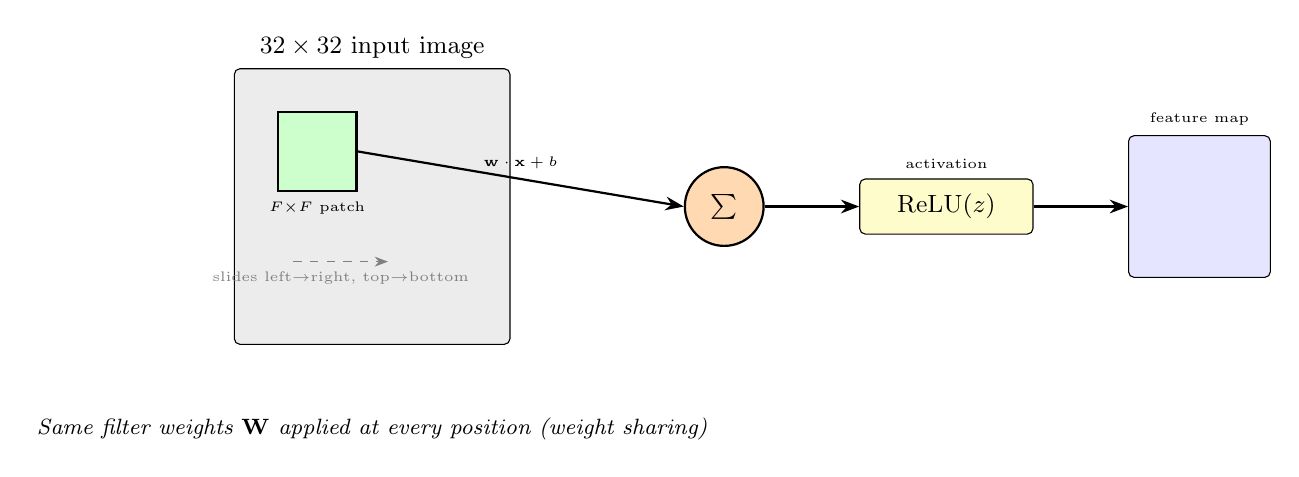
\begin{tikzpicture}[
  >=Stealth,
  every node/.style={font=\small},
  box/.style={draw, minimum width=1.2cm, minimum height=1.2cm,
              fill=gray!15, rounded corners=2pt},
  patch/.style={draw, thick, minimum width=1.0cm, minimum height=1.0cm,
                fill=green!20},
  neuron/.style={draw, circle, minimum size=1.0cm,
                 fill=orange!30, thick},
  outbox/.style={draw, minimum width=2.2cm, minimum height=0.7cm,
                 fill=yellow!20, rounded corners=2pt}
]
%% input image
\node[box, minimum width=3.5cm, minimum height=3.5cm,
      label=above:{$32\times32$ input image}] (img) at (0,0) {};
%% patch highlight
\node[patch] (patch) at (-0.7,0.7) {};
\node[font=\tiny, below=0pt of patch] {$F{\times}F$ patch};
%% arrow from patch to neuron
\node[neuron, right=2.2cm of img] (neur) {$\sum$};
\draw[->, thick] (patch.east) -- node[above, font=\tiny]{$\mathbf{w}\cdot\mathbf{x}+b$} (neur.west);
%% activation
\node[outbox, right=1.2cm of neur, label=above:{\tiny activation}] (act) {$\relu(z)$};
\draw[->, thick] (neur) -- (act);
%% feature map
\node[box, minimum width=1.8cm, minimum height=1.8cm,
      right=1.2cm of act, fill=blue!10,
      label=above:{\tiny feature map}] (fm) {};
\draw[->, thick] (act) -- (fm);
%% sliding arrow
\draw[->, dashed, gray] (-1.0,-0.7) -- node[below, font=\tiny]{slides left$\to$right, top$\to$bottom} (0.2,-0.7);
%% label
\node[below=0.8cm of img, font=\footnotesize\itshape]
  {Same filter weights $\mathbf{W}$ applied at every position (weight sharing)};
\end{tikzpicture}
\caption{Convolution as a neuron with a local receptive field.
         The filter $\mathbf{W}$ (size $F\times F$) slides across the input
         image, computing a dot product at each position to produce one element
         of the output feature map.  ReLU is applied after each dot product.}
\label{fig:conv_neuron}
\end{figure}

\subsection{Multiple Filters and Multiple Feature Maps}
\label{subsec:multi_filter}

A single convolutional layer typically applies $K$ independent filters
$\mathbf{W}^{(1)}, \ldots, \mathbf{W}^{(K)}$ to the same input.  Each filter
produces one feature map, so the layer output is a 3-D tensor of shape
$(K, N_{\text{out}}, N_{\text{out}})$.  The number of feature maps equals the
number of filters:

\begin{equation}
  \text{number of output feature maps} = K.
  \label{eq:num_fm}
\end{equation}

A common design principle is to \emph{increase} $K$ with depth, compensating
for the spatial shrinkage caused by successive convolution and pooling
operations.

% ══════════════════════════════════════════════════════════════════════════════
\section{Block Diagram of the CNN Architecture}
\label{sec:block_diagram}
% ══════════════════════════════════════════════════════════════════════════════

\subsection{Overall Pipeline}
\label{subsec:overall_pipeline}

A canonical CNN for image classification consists of two sequential modules:

\begin{enumerate}[label=\arabic*.]
  \item \textbf{Feature extractor:} one or more repetitions of
        $(\text{Conv} + \relu) \to \text{Pooling}$.
  \item \textbf{Classifier:} Flatten $\to$ one or more fully connected layers
        $\to$ Softmax output.
\end{enumerate}

Each CNN ``layer'' is itself a three-stage block:

\begin{description}[leftmargin=3em, style=nextline]
  \item[Stage 1 -- Convolution] The filter slides over the input performing
        element-wise multiplication and summation, producing an activation
        map.
  \item[Stage 2 -- Non-linearity] ReLU is applied element-wise:
        $\relu(x) = \max(0, x)$.  This zeroes negative activations and
        introduces the non-linearity required for the network to learn complex
        functions.
  \item[Stage 3 -- Pooling] A pooling window (typically $2\times2$) slides
        over the feature map and retains only the most salient value (max
        pooling) or an aggregate (average pooling), reducing spatial
        dimensions and providing translation invariance.
\end{description}

\subsection{TikZ Diagram: CNN Block Diagram}
\label{subsec:block_tikz}

\Cref{fig:cnn_block} shows the full CNN pipeline from input image to softmax
output.

\begin{figure}[ht]
\centering
\resizebox{\textwidth}{!}{%
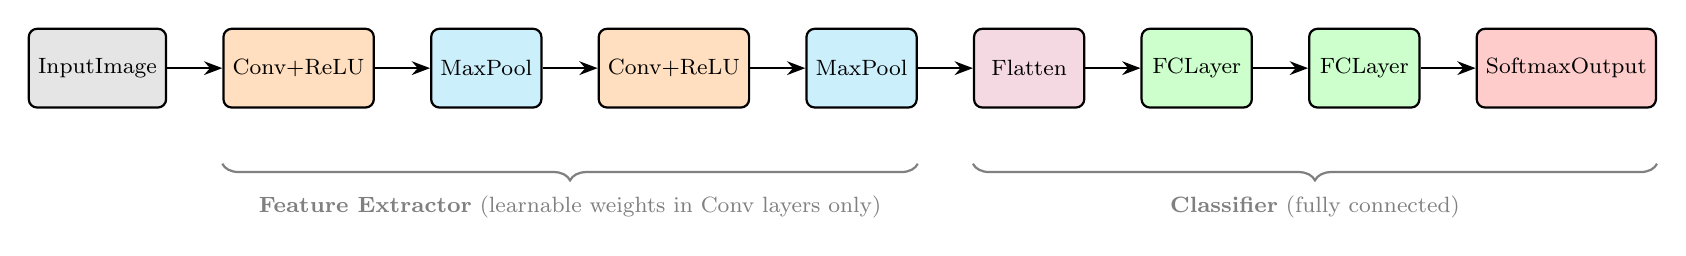
\begin{tikzpicture}[
  >=Stealth,
  every node/.style={font=\footnotesize},
  blk/.style={draw, rounded corners=3pt, minimum width=1.4cm,
              minimum height=1.0cm, text centered, thick},
  arr/.style={->, thick}
]
%% Nodes
\node[blk, fill=gray!20]                               (inp)  {Input\\Image};
\node[blk, fill=orange!25,  right=0.7cm of inp]        (c1)   {Conv\\+ReLU};
\node[blk, fill=cyan!20,    right=0.7cm of c1]         (p1)   {Max\\Pool};
\node[blk, fill=orange!25,  right=0.7cm of p1]         (c2)   {Conv\\+ReLU};
\node[blk, fill=cyan!20,    right=0.7cm of c2]         (p2)   {Max\\Pool};
\node[blk, fill=purple!15,  right=0.7cm of p2]         (fl)   {Flatten};
\node[blk, fill=green!20,   right=0.7cm of fl]         (fc1)  {FC\\Layer};
\node[blk, fill=green!20,   right=0.7cm of fc1]        (fc2)  {FC\\Layer};
\node[blk, fill=red!20,     right=0.7cm of fc2]        (sm)   {Softmax\\Output};

%% Arrows
\draw[arr] (inp) -- (c1);
\draw[arr] (c1)  -- (p1);
\draw[arr] (p1)  -- (c2);
\draw[arr] (c2)  -- (p2);
\draw[arr] (p2)  -- (fl);
\draw[arr] (fl)  -- (fc1);
\draw[arr] (fc1) -- (fc2);
\draw[arr] (fc2) -- (sm);

%% Braces / labels below
\draw[decorate, decoration={brace,amplitude=6pt,mirror},
      thick, gray]
  ([yshift=-0.7cm]c1.south west) -- ([yshift=-0.7cm]p2.south east)
  node[midway, below=8pt] {\textbf{Feature Extractor} (learnable weights in Conv layers only)};

\draw[decorate, decoration={brace,amplitude=6pt,mirror},
      thick, gray]
  ([yshift=-0.7cm]fl.south west) -- ([yshift=-0.7cm]sm.south east)
  node[midway, below=8pt] {\textbf{Classifier} (fully connected)};
\end{tikzpicture}}
\caption{Block diagram of a CNN with two convolution--pooling stages followed
         by fully-connected classification layers.  The pooling layers have no
         learnable weights; only the convolutional and fully-connected layers
         participate in backpropagation.}
\label{fig:cnn_block}
\end{figure}

\subsection{Where Are the Neurons?}
\label{subsec:where_neurons}

A natural question is: where do neurons appear in the CNN pipeline?

\begin{itemize}[leftmargin=2em]
  \item \textbf{Convolution layer:} every output element $a_{i,j}^{(k)}$ is
        produced by a neuron-like operation (weighted sum $+$ bias $+$
        activation).  Weights \emph{are} learned here via backpropagation.
  \item \textbf{Pooling layer:} no weighted sum, no learnable weights.  This
        is a fixed aggregation operation (max / average).  No
        backpropagation through learnable parameters occurs here.
  \item \textbf{Flatten layer:} purely a shape transformation (2-D
        $\to$ 1-D); no learnable parameters.
  \item \textbf{Fully connected layers:} standard neurons, each connected to
        all elements of the preceding feature vector.
\end{itemize}

\begin{remark}
Pooling is an \emph{optional} layer.  Modern architectures (e.g.\
ResNets) sometimes use strided convolutions instead of pooling to reduce
spatial dimensions, or omit pooling entirely in certain stages.
\end{remark}

% ══════════════════════════════════════════════════════════════════════════════
\section{Convolution Output Size Formula}
\label{sec:output_size}
% ══════════════════════════════════════════════════════════════════════════════

\subsection{Derivation}
\label{subsec:derivation}

Consider a 1-D input of length $N$, a filter of size $F$, and a stride of
$S$.  Starting at position $0$, the filter can be placed at positions
$0, S, 2S, \ldots$ as long as the filter does not exceed the input boundary.
The last valid start position is $N - F$, which is reached in
$\lfloor(N-F)/S\rfloor$ steps.  Including the initial position, the total
number of valid placements -- equivalently, the output size -- is

\begin{equation}
  \boxed{N_{\text{out}} = \left\lfloor \frac{N - F}{S} \right\rfloor + 1.}
  \label{eq:output_size}
\end{equation}

For integer outputs this requires $(N - F)$ to be divisible by $S$.  When
this condition is not met, PyTorch raises a runtime error.

\subsection{Effect of Zero-Padding}
\label{subsec:padding}

Zero-padding adds $P$ rows (and columns) of zeros around the input, making
the effective input size $N + 2P$.  \Cref{eq:output_size} becomes

\begin{equation}
  N_{\text{out}} = \left\lfloor \frac{N + 2P - F}{S} \right\rfloor + 1.
  \label{eq:output_size_pad}
\end{equation}

Setting $P = (F-1)/2$ (``same'' padding, valid for odd $F$ with $S=1$)
ensures $N_{\text{out}} = N$, i.e.\ the feature map has the same spatial
dimensions as the input.

\begin{definition}[Valid Convolution Configuration]
\label{def:valid_config}
A combination $(N, F, S)$ is \emph{valid} if and only if $(N - F)$ is
exactly divisible by $S$, i.e.\ $(N - F) \bmod S = 0$.
\end{definition}

\subsection{Worked Examples (from the Lecture)}
\label{subsec:worked_examples}

The instructor worked through the following three cases using a
$7\times7$ input and a $3\times3$ filter:

\begin{table}[ht]
\centering
\caption{Output size for a $7\times7$ input with $3\times3$ filter at varying
         strides. Only integer outputs are valid.}
\label{tab:stride_examples}
\begin{tabular}{cccc}
\toprule
\textbf{Input ($N$)} & \textbf{Filter ($F$)} & \textbf{Stride ($S$)} &
\textbf{Output size} \\
\midrule
7 & 3 & 1 & $(7-3)/1 + 1 = \mathbf{5}$ \quad (valid) \\
7 & 3 & 2 & $(7-3)/2 + 1 = \mathbf{3}$ \quad (valid) \\
7 & 3 & 3 & $(7-3)/3 + 1 = 2.33\ldots$ \quad \textbf{invalid} \\
\bottomrule
\end{tabular}
\end{table}

\begin{warningbox}
If $(N-F)/S$ is not an integer, the convolution is \textbf{invalid}.  PyTorch
will raise a \texttt{RuntimeError} and refuse to run the forward pass.
Never assume that any combination of input size, filter size, and stride will
work -- always verify with \cref{eq:output_size} before building the model.
\end{warningbox}

\subsection{Applying the Formula: $32\times32$ Input with $5\times5$ Filter}
\label{subsec:formula_32}

The lecture uses this example to explain why the first feature map in the
canonical CNN diagram has spatial size $28\times28$:

\begin{align}
  N &= 32, \quad F = 5, \quad S = 1, \quad P = 0 \notag \\
  N_{\text{out}} &= \frac{32 - 5}{1} + 1 = 28.
  \label{eq:32to28}
\end{align}

\begin{example}
\textbf{Verifying the $7\times7 \to 5\times5$ case.}

Input: $7\times7$; filter: $3\times3$; stride: $1$.
\[
  N_{\text{out}} = \frac{7 - 3}{1} + 1 = 5.
\]
The filter can scan 5 positions left-to-right and 5 positions top-to-bottom,
producing a $5\times5$ output matrix with exactly 25 scalar values.
\end{example}

% ══════════════════════════════════════════════════════════════════════════════
\section{Pooling Operations}
\label{sec:pooling}
% ══════════════════════════════════════════════════════════════════════════════

\subsection{Max Pooling}
\label{subsec:max_pool}

Max pooling slides a window of size $P_w \times P_w$ over the feature map
with stride $S_p$ and retains the maximum value in each window:

\begin{equation}
  y_{i,j} = \max_{0 \le p < P_w,\; 0 \le q < P_w}
             a_{iS_p + p,\; jS_p + q}.
  \label{eq:maxpool}
\end{equation}

A $2\times2$ window with stride $2$ halves both spatial dimensions, so a
$28\times28$ feature map becomes $14\times14$.

\subsection{Average Pooling}
\label{subsec:avg_pool}

Average pooling replaces the $\max$ in \cref{eq:maxpool} with the arithmetic
mean:
\begin{equation}
  y_{i,j} = \frac{1}{P_w^2}
             \sum_{p=0}^{P_w-1}\sum_{q=0}^{P_w-1}
             a_{iS_p + p,\; jS_p + q}.
  \label{eq:avgpool}
\end{equation}

\subsection{Why Pooling Provides Translation Invariance}
\label{subsec:pool_invariance}

If a feature (e.g.\ a detected edge) shifts by one pixel, the max-pooling
window may still capture the same maximum value.  Repeated pooling layers
accumulate this robustness, so that the final feature vector is approximately
invariant to small spatial translations of the input.

\begin{keyinsight}[title=Key Insight: Translation Invariance]
Max pooling retains the strongest activation within each local window,
regardless of its precise position.  After two pooling layers, the CNN
``knows'' that a feature is present in a neighbourhood, not at a specific
pixel.  This is why CNNs generalise better to translated images than FFNNs
(see \cref{tab:cnn_vs_ffnn}).
\end{keyinsight}

\subsection{Pooling Output Size}
\label{subsec:pool_size}

The output size formula for pooling is the same as for convolution,
\cref{eq:output_size}, with $N \leftarrow N_{\text{feature map}}$,
$F \leftarrow P_w$, and $S \leftarrow S_p$.  With $P_w = 2$ and $S_p = 2$:

\begin{equation}
  N_{\text{pool}} = \frac{N_{\text{feature map}} - 2}{2} + 1
                  = \frac{N_{\text{feature map}}}{2}.
  \label{eq:pool_size}
\end{equation}

\subsection{Comparing Convolution and Pooling Layers}

\begin{table}[ht]
\centering
\caption{Comparison of convolutional and pooling layers.}
\label{tab:conv_vs_pool}
\begin{tabular}{lcc}
\toprule
\textbf{Property} & \textbf{Convolution Layer} & \textbf{Pooling Layer} \\
\midrule
Operation & Weighted sum $+$ bias & Max / average \\
Learnable weights & Yes & No \\
Activation function & Yes (ReLU) & No \\
Spatial size change & Reduces by $(F-1)/S$ & Reduces by factor $S_p$ \\
Feature channels & Increases (more filters) & Unchanged \\
Participates in backprop & Yes & No (fixed) \\
Optional in CNN & No (core layer) & Yes (can be skipped) \\
\bottomrule
\end{tabular}
\end{table}

% ══════════════════════════════════════════════════════════════════════════════
\section{Hierarchical Feature Learning}
\label{sec:hierarchical}
% ══════════════════════════════════════════════════════════════════════════════

A deep CNN extracts features at increasing levels of abstraction:

\begin{enumerate}[label=\textbf{Layer \arabic*:}]
  \item \textbf{Low-level features} -- horizontal edges, vertical edges,
        diagonal edges, colour blobs.  These are detected by the first
        convolution layer's filters, whose receptive field is small (e.g.\
        $3\times3$).
  \item \textbf{Mid-level features} -- combinations of edges forming corners,
        textures, simple shapes.  The second convolution layer's filters see
        the output of the first pooling layer and can combine primitives over
        a larger effective receptive field.
  \item \textbf{High-level features} -- object parts (e.g.\ wheel shape, eye
        pattern, fur texture).  Deeper layers accumulate evidence from wider
        input regions.
  \item \textbf{Classification} -- the fully connected head receives a
        flattened high-level feature vector and maps it to class logits via
        learned linear transformations, with a softmax at the output.
\end{enumerate}

\begin{remark}
The filter weights that produce these hierarchical features are never
manually designed.  They are initialised randomly and learnt entirely through
backpropagation on labelled training data.  The ``edge detectors'' in early
layers emerge automatically as the most useful low-level basis for the task.
\end{remark}

% ══════════════════════════════════════════════════════════════════════════════
\section{Spatial Dimensions: A Closer Look}
\label{sec:spatial}
% ══════════════════════════════════════════════════════════════════════════════

\subsection{Stride and Feature Resolution}
\label{subsec:stride_resolution}

Stride controls the resolution of the output feature map:

\begin{itemize}[leftmargin=2em]
  \item \textbf{Stride $= 1$:} the filter visits every pixel.  All fine-grained
        spatial detail is captured.  Preferred when every local feature is
        important.
  \item \textbf{Stride $= 2$:} the filter skips alternate positions.  Spatial
        resolution is halved.  Some fine detail is lost, but computation is
        reduced by $4\times$ (fewer output elements).
  \item \textbf{Stride $> 2$:} increasingly coarse feature maps.  Used in
        the first layer of large-scale models (e.g.\ AlexNet uses stride 4
        on the first $11\times11$ layer) to rapidly reduce the spatial footprint
        of a high-resolution input.
\end{itemize}

\begin{example}
\textbf{Effect of stride on a $7\times7$ input with $3\times3$ filter.}
\begin{align*}
  S=1: &\quad N_{\text{out}} = (7-3)/1 + 1 = 5. \quad \text{fine-grained} \\
  S=2: &\quad N_{\text{out}} = (7-3)/2 + 1 = 3. \quad \text{coarser} \\
  S=3: &\quad N_{\text{out}} = (7-3)/3 + 1 = 2.33\ldots \quad
              \text{\textbf{invalid}} \\
\end{align*}
With stride~3, the filter cannot tile the $7\times7$ grid cleanly.  After the
second placement the filter would require a third column that does not exist
(only 1 column remains, but 3 are needed for the filter).
\end{example}

\subsection{Design Rule for Valid Configurations}
\label{subsec:valid_rule}

\begin{theorem}[Valid Stride Condition]
\label{thm:valid_stride}
A convolution on a spatial dimension of size $N$ with filter size $F$ and
stride $S$ (and no padding) is valid if and only if
\begin{equation}
  (N - F) \bmod S = 0.
  \label{eq:valid_cond}
\end{equation}
\end{theorem}

\begin{proof}
The filter must reach position $N-F$ (the last valid starting position) in an
integer number of stride steps from position $0$.  This requires
$(N-F) / S \in \mathbb{Z}_{\geq 0}$, i.e.\ $(N-F)$ divisible by $S$.
\end{proof}

% ══════════════════════════════════════════════════════════════════════════════
\section{PyTorch Implementation of a Two-Layer CNN}
\label{sec:pytorch}
% ══════════════════════════════════════════════════════════════════════════════

\subsection{Dataset: Fashion-MNIST}
\label{subsec:dataset}

The session uses the Fashion-MNIST dataset (\texttt{04-DL-CNN} Colab notebook):
\begin{itemize}[leftmargin=2em]
  \item 60\,000 training images $+$ 10\,000 test images.
  \item Each image: $28\times28$ grayscale pixels, 10 classes
        (T-shirt, trouser, pullover, dress, coat, sandal, shirt, sneaker,
        bag, ankle boot).
  \item Original CSV format: each row is one flattened image (784 pixel
        values) with a label in the first column.
\end{itemize}

For the CNN, the 784-element rows are \textbf{reshaped} to
$(1, 28, 28)$ tensors (batch dimension is handled by the DataLoader):
\begin{equation}
  \text{shape} = (\text{batch\_size},\; C_{\text{in}},\; H,\; W)
               = (\text{-}1,\; 1,\; 28,\; 28).
  \label{eq:data_shape}
\end{equation}

\subsection{Network Architecture}
\label{subsec:architecture}

The CNN defined in the notebook has the following structure:

\paragraph{Feature Extractor (Sequential container 1)}
\begin{enumerate}[label=\textbf{\arabic*.}]
  \item \texttt{Conv2d}(in\_channels=1, out\_channels=32,
        kernel\_size=3, stride=1, padding=``same'', bias=True)
  \item \texttt{ReLU}
  \item \texttt{BatchNorm2d}(32)
  \item \texttt{MaxPool2d}(kernel\_size=2, stride=2)
        \hfill $28\times28 \to 14\times14$
  \item \texttt{Conv2d}(in\_channels=32, out\_channels=64,
        kernel\_size=3, stride=1, padding=``same'', bias=True)
  \item \texttt{ReLU}
  \item \texttt{BatchNorm2d}(64)
  \item \texttt{MaxPool2d}(kernel\_size=2, stride=2)
        \hfill $14\times14 \to 7\times7$
\end{enumerate}

\paragraph{Classifier (Sequential container 2, after Flatten)}
\begin{enumerate}[label=\textbf{\arabic*.}]
  \item \texttt{Linear}($64\times7\times7 = 3136 \to 128$)
  \item \texttt{ReLU}
  \item \texttt{Linear}($128 \to 64$)
  \item \texttt{ReLU}
  \item \texttt{Linear}($64 \to 10$)
\end{enumerate}

\subsection{Parameter Count Analysis}
\label{subsec:param_count}

\Cref{tab:param_count} summarises the learnable parameters per layer.

\begin{table}[ht]
\centering
\caption{Learnable parameter count for each layer of the CNN.}
\label{tab:param_count}
\begin{tabular}{lrr}
\toprule
\textbf{Layer} & \textbf{Shape} & \textbf{Parameters} \\
\midrule
Conv2d-1 (weights) & $32\times1\times3\times3$ & 288 \\
Conv2d-1 (bias)    & $32$                       & 32  \\
BatchNorm2d-1      & $2\times32$                & 64  \\
Conv2d-2 (weights) & $64\times32\times3\times3$ & 18\,432 \\
Conv2d-2 (bias)    & $64$                       & 64  \\
BatchNorm2d-2      & $2\times64$                & 128 \\
Linear-1           & $3136\times128$            & 401\,408 \\
Linear-1 (bias)    & $128$                      & 128 \\
Linear-2           & $128\times64$              & 8\,192 \\
Linear-2 (bias)    & $64$                       & 64  \\
Linear-3           & $64\times10$               & 640 \\
Linear-3 (bias)    & $10$                       & 10  \\
\midrule
\textbf{Total (approx.)} & & $\sim$\,3\,142 \\
\bottomrule
\end{tabular}
\end{table}

\subsection{Training Algorithm}
\label{subsec:training}

\begin{algorithm}[H]
\caption{Mini-Batch Training of CNN (Fashion-MNIST)}
\label{alg:cnn_train}
\DontPrintSemicolon
\SetAlgoLined
\KwIn{Training set $\mathcal{D}_{\text{train}}$, batch size $B=32$,
      epochs $T$, learning rate $\eta$, weight decay $\lambda$}
\KwOut{Trained CNN parameters $\theta$}

Initialise $\theta$ randomly (Kaiming uniform for Conv/Linear)\;
\For{$t = 1$ \KwTo $T$}{
  \ForEach{mini-batch $(X_b, y_b)$ from $\mathcal{D}_{\text{train}}$}{
    Reshape $X_b$ to shape $(B, 1, 28, 28)$\;
    \tcp{Forward pass}
    $\hat{y}_b \leftarrow \mathrm{CNN}_\theta(X_b)$
    \tcp*{logits, shape $(B, 10)$}
    $\mathcal{L} \leftarrow \mathrm{CrossEntropy}(\hat{y}_b,\, y_b)$\;
    \tcp{Backward pass}
    Zero gradients: $\nabla_\theta \leftarrow \mathbf{0}$\;
    $\nabla_\theta \leftarrow \partial\mathcal{L}/\partial\theta$
    \tcp*{backpropagation}
    \tcp{Parameter update (Adam with weight decay)}
    $\theta \leftarrow \theta - \eta\,\nabla_\theta - \eta\lambda\,\theta$\;
  }
  Evaluate on validation set; log accuracy\;
}
\Return $\theta$\;
\end{algorithm}

% ══════════════════════════════════════════════════════════════════════════════
\section{CNN vs.\ FFNN: Comparative Results}
\label{sec:results}
% ══════════════════════════════════════════════════════════════════════════════

\subsection{Experimental Setup}
\label{subsec:exp_setup}

Both models are trained on the Fashion-MNIST \emph{two-class} subset
(binary classification) to make the comparison controlled.  The same
training procedure (Adam optimiser, same number of epochs, same batch size)
is applied to both models.  Two evaluation conditions are used:

\begin{enumerate}[label=\arabic*.]
  \item \textbf{Original images:} test set without any augmentation.
  \item \textbf{Translated images:} test images shifted by a few pixels,
        simulating a distribution shift that breaks spatial position
        assumptions.
\end{enumerate}

\subsection{Results Table}
\label{subsec:results_table}

\begin{table}[ht]
\centering
\caption{CNN vs.\ FFNN: parameter count and test accuracy on original
         and translated Fashion-MNIST images (two-class subset).}
\label{tab:cnn_vs_ffnn}
\begin{tabular}{lrcc}
\toprule
\multirow{2}{*}{\textbf{Model}} &
\multirow{2}{*}{\textbf{Parameters}} &
\multicolumn{2}{c}{\textbf{Test Accuracy}} \\
\cmidrule(lr){3-4}
 & & \textbf{Original} & \textbf{Translated} \\
\midrule
FFNN  & 39\,352 & 96.47\,\%  & 80.42\,\% \\
CNN   & 3\,142  & $\approx$98\,\%  & 88.26\,\% \\
\midrule
\textbf{Improvement} & $12\times$ fewer & $+1.5$\,pp & $+7.8$\,pp \\
\bottomrule
\end{tabular}
\end{table}

\subsection{Analysis of Results}
\label{subsec:analysis}

\Cref{tab:cnn_vs_ffnn} reveals three important findings:

\begin{enumerate}[label=\arabic*.]
  \item \textbf{Parameter efficiency.}  The CNN achieves better accuracy
        with $12\times$ fewer parameters ($3\,142$ vs.\ $39\,352$).  This
        results directly from weight sharing in convolutional layers: a
        $3\times3$ filter has only 9 weights regardless of input size.
  \item \textbf{Higher accuracy on original images.}  CNN reaches
        $\approx 98\,\%$ vs.\ FFNN's $96.47\,\%$.  Exploiting spatial
        structure leads to better feature representations.
  \item \textbf{Dramatically better generalisation to translated images.}
        CNN achieves $88.26\,\%$ vs.\ FFNN's $80.42\,\%$ on translated
        inputs -- a gap of $7.8$ percentage points.  This confirms the
        translation invariance benefit of max-pooling layers.
\end{enumerate}

\begin{keyinsight}[title=Key Insight: Why CNN Handles Translation]
FFNN memorises the exact pixel positions of features.  When an image is
shifted, the pixel values appear at new indices and the FFNN ``sees'' an
unfamiliar pattern.  The CNN's pooling layers aggregate over small
neighbourhoods, making the representation robust to small shifts.
\end{keyinsight}

% ══════════════════════════════════════════════════════════════════════════════
\section{Live Visualisation: Convolution and Pooling in Action}
\label{sec:visualisation}
% ══════════════════════════════════════════════════════════════════════════════

During the session the instructor demonstrated convolution using the
\texttt{deeplizard} interactive visualisation website with Fashion-MNIST
images.  Key observations:

\begin{enumerate}[label=\arabic*.]
  \item \textbf{Filter sliding:} the $3\times3$ window moves left-to-right,
        top-to-bottom across the image with stride~1.  At each position, nine
        element-wise multiplications are summed to give one output scalar.
  \item \textbf{Edge detection:} a ``top-edge'' filter (weights structured to
        respond to horizontal transitions) produces high (positive, red)
        activations at top edges and low (negative, blue) activations
        elsewhere.
  \item \textbf{ReLU effect:} all negative (blue) values are zeroed by ReLU,
        leaving only the detected edge features.
  \item \textbf{Filter direction:} swapping to a ``right-edge'' filter
        shifts the strong activations to the right side of the image,
        confirming that filter weights determine what feature is extracted.
  \item \textbf{Learnt filters:} in a real CNN, filter weights are not
        hand-designed.  They are initialised randomly and optimised via
        backpropagation; the network learns which features are useful for
        the task.
  \item \textbf{Max pooling:} the pooling demo showed a $2\times2$ window
        with stride~2.  Each window retains its maximum; a $4\times4$ feature
        map is reduced to $2\times2$.
\end{enumerate}

% ══════════════════════════════════════════════════════════════════════════════
\section{Design Choices and Hyperparameters}
\label{sec:design}
% ══════════════════════════════════════════════════════════════════════════════

\subsection{Choosing the Number of Filters}
\label{subsec:num_filters}

Selecting the number of filters per layer is more art than science:

\begin{itemize}[leftmargin=2em]
  \item There is no analytic formula for the optimal number of filters.
  \item A common heuristic: \emph{increase} the number of filters as depth
        increases, to compensate for the shrinking spatial dimensions and
        prevent information bottlenecks.  The lecture example uses 32 filters
        in layer~1 and 64 in layer~2.
  \item The practical approach is to start with a reasonable number and tune
        by observing validation accuracy.
\end{itemize}

\subsection{Kernel / Filter Terminology}
\label{subsec:terminology}

The terms \emph{kernel} and \emph{filter} are often used interchangeably in
the literature.  One useful convention adopted in the lecture:

\begin{itemize}[leftmargin=2em]
  \item \textbf{Kernel:} the weight matrix itself (e.g.\ a $3\times3$ array
        of floats).
  \item \textbf{Filter:} a collection of kernels -- one per input channel --
        that together produce one output feature map.  For a 3-channel (RGB)
        input with a $5\times5$ kernel, each filter contains
        $3 \times 5 \times 5 = 75$ weights.
\end{itemize}

\subsection{Choosing Stride}
\label{subsec:choosing_stride}

\begin{itemize}[leftmargin=2em]
  \item \textbf{Stride 1:} maximum feature resolution.  Recommended when
        the image contains dense information throughout (e.g.\ texture
        classification, medical imaging).
  \item \textbf{Stride 2:} halves the feature map size, reducing memory and
        computation.  Commonly used in pooling layers and sometimes in strided
        convolutions as a pooling substitute.
  \item Always verify that $(N - F) \bmod S = 0$ before training; otherwise
        PyTorch will raise an error.
\end{itemize}

% ══════════════════════════════════════════════════════════════════════════════
\section{Connecting Convolution to the Full CNN Forward Pass}
\label{sec:forward_pass}
% ══════════════════════════════════════════════════════════════════════════════

\subsection{Dimension Trace Through the Network}
\label{subsec:dim_trace}

Starting from a single $28\times28$ grayscale image, the spatial and channel
dimensions evolve as follows through the two-layer CNN:

\begin{align}
  \text{Input:} &\quad (1,\; 28,\; 28) \notag \\
  \text{After Conv2d-1 (same padding):} &\quad (32,\; 28,\; 28) \notag \\
  \text{After MaxPool2d (2, stride=2):} &\quad (32,\; 14,\; 14) \notag \\
  \text{After Conv2d-2 (same padding):} &\quad (64,\; 14,\; 14) \notag \\
  \text{After MaxPool2d (2, stride=2):} &\quad (64,\; 7,\; 7) \notag \\
  \text{After Flatten:} &\quad (3136,) \notag \\
  \text{After Linear-1:} &\quad (128,) \notag \\
  \text{After Linear-2:} &\quad (64,) \notag \\
  \text{After Linear-3 (logits):} &\quad (10,) \notag \\
  \text{After Softmax:} &\quad (10,) \quad \text{probabilities}
  \label{eq:dim_trace}
\end{align}

The flatten step converts the $(64, 7, 7)$ tensor to a $64\times7\times7 =
3136$-dimensional vector before the first linear layer.

\subsection{Cross-Entropy Loss}
\label{subsec:loss}

The network is trained with cross-entropy loss:
\begin{equation}
  \mathcal{L} = -\sum_{c=1}^{C} y_c \log \hat{p}_c,
  \label{eq:crossentropy}
\end{equation}
where $y_c \in \{0,1\}$ is the one-hot true label and $\hat{p}_c$ is the
predicted probability for class $c$.  Backpropagation computes gradients of
$\mathcal{L}$ with respect to all learnable parameters (Conv and Linear
weights and biases; BatchNorm scale and shift), which are then updated by the
Adam optimiser.

% ══════════════════════════════════════════════════════════════════════════════
\section{Summary and Conclusions}
\label{sec:summary}
% ══════════════════════════════════════════════════════════════════════════════

\subsection{Lecture Summary}
\label{subsec:lecture_summary}

Session~13 provided a comprehensive hands-on treatment of Convolutional
Neural Networks, covering:

\begin{enumerate}[label=\arabic*., leftmargin=2.5em]
  \item \textbf{Conceptual foundation:} A convolutional filter is a neuron
        applied locally, performing the same $\mathbf{w}\cdot\mathbf{x}+b$
        computation as any fully connected neuron, but restricted to a small
        receptive field and with weights shared across all spatial positions.
  \item \textbf{CNN architecture:} the three-stage layer structure
        (Conv $\to$ ReLU $\to$ Pooling), the flatten bridge, and the
        fully-connected classifier.
  \item \textbf{Output-size formula:}
        $N_{\text{out}} = \lfloor(N-F)/S\rfloor + 1$, with the validity
        condition $(N-F) \bmod S = 0$ enforced by PyTorch at runtime.
  \item \textbf{Worked examples} for a $7\times7$ input with a $3\times3$
        filter at strides 1, 2, and 3 (the last being invalid).
  \item \textbf{Pooling:} max pooling as a fixed aggregation operation that
        reduces spatial dimensions and introduces translation invariance.
        No learnable weights; optional but strongly recommended.
  \item \textbf{PyTorch implementation:} two convolutional blocks
        ($32$~filters then $64$~filters) followed by a three-layer
        fully-connected classifier, yielding $\sim$3\,142 total parameters.
  \item \textbf{Comparative results:} CNN achieves $\approx98\,\%$ accuracy
        on original images and $88.26\,\%$ on translated images, versus
        $96.47\,\%$ and $80.42\,\%$ for the FFNN -- with $12\times$ fewer
        parameters.
\end{enumerate}

\subsection{Key Takeaways}
\label{subsec:takeaways}

\begin{keyinsight}[title=Key Takeaway 1 -- Parameter Efficiency]
Weight sharing in convolutional layers is the primary mechanism behind CNN's
dramatic parameter reduction.  A $3\times3$ filter has only 9 weights
regardless of input size, compared to $N^2$ weights for a fully connected
neuron on an $N\times N$ image.
\end{keyinsight}

\begin{keyinsight}[title=Key Takeaway 2 -- Translation Invariance]
Max-pooling layers aggregate the strongest activations over local
neighbourhoods, making the feature representation approximately invariant to
small translations.  This is directly reflected in the results: CNN drops only
$\sim$10 pp on translated images versus $\sim$16 pp for FFNN.
\end{keyinsight}

\begin{keyinsight}[title=Key Takeaway 3 -- Validity of Configurations]
Not all combinations of input size, filter size, and stride are valid.  Always
verify $(N-F)\bmod S = 0$ before committing to a network architecture.  Use
``same'' padding when you want the feature map to match the input size.
\end{keyinsight}

\subsection{Looking Ahead}
\label{subsec:ahead}

The session explicitly noted that CNN material will continue for one or two
more sessions, covering:

\begin{itemize}[leftmargin=2em]
  \item Deeper and more complex CNN architectures (beyond two conv layers).
  \item \texttt{Conv1d} for sequential / text data.
  \item Possibly canonical architectures such as LeNet, AlexNet, or VGGNet.
  \item Full 10-class Fashion-MNIST CNN results.
\end{itemize}

\vspace{1.5em}
\noindent\rule{\textwidth}{0.5pt}\\[0.3em]
{\small\itshape
These notes are derived from the recorded lecture available at
\url{https://vimeo.com/1151039438} and the slides at
\url{https://learning.iiitdwd.ac.in/mod/pdfprotect/view.php?id=1390}.
All mathematical derivations follow the content presented by the instructor.}

\clearpage

%% ============================================================
%% Session 14: CNN Architectures: AlexNet, VGGNet, and ResNet
%% ============================================================
\part{Session 14: CNN Architectures: AlexNet, VGGNet, and ResNet}

% -------------------------------------------------------
%  TITLE PAGE
% -------------------------------------------------------
\begin{titlepage}
  \centering
  \vspace*{2cm}
  {\LARGE\bfseries Deep Learning\par}
  \vspace{0.5cm}
  {\large Session 14 Lecture Notes\par}
  \vspace{1.5cm}
  {\huge\bfseries Popular CNN Architectures\\[0.4em]
   AlexNet, VGGNet, and ResNet\par}
  \vspace{1.5cm}
  {\large
    \textbf{Instructors:} Prof.\ S R M Prasanna \& Dr.\ Sunil Saumya\\[0.3em]
    Indian Institute of Information Technology Dharwad (IIIT-DWD)\\[0.3em]
    \textbf{Deck:} \texttt{07\_DL\_Popular CNN Architectures}\\[0.3em]
    \textbf{Duration:} $\approx$1 hour 44 minutes\\[0.3em]
    \textbf{Video:} \url{https://vimeo.com/1151649038}
  }
  \vfill
  {\large\today\par}
\end{titlepage}

% -------------------------------------------------------
%  TABLE OF CONTENTS
% -------------------------------------------------------

\newpage

% -------------------------------------------------------
%  1. INTRODUCTION
% -------------------------------------------------------
\section{Introduction}
\label{sec:intro}

The year 2012 marked a watershed moment in the history of computer vision and artificial intelligence. Prior to that year, the state of the art on the ImageNet Large Scale Visual Recognition Challenge (ILSVRC) hovered around a top-5 error rate of $26\%$, achieved by carefully hand-engineered feature pipelines. A single result -- a convolutional neural network trained on two NVIDIA GTX 580 GPUs -- obliterated this benchmark, achieving $15.3\%$ top-5 error and launching the modern era of deep learning.

Session 14 surveys the three landmark CNN architectures that defined this progression:
\begin{enumerate}[leftmargin=2em]
  \item \textbf{AlexNet} (Krizhevsky et al., NIPS 2012) -- demonstrated that deep CNNs could outperform all prior hand-crafted methods on ImageNet by a wide margin.
  \item \textbf{VGGNet} (Simonyan \& Zisserman, ICLR 2015) -- systematically showed that depth, using exclusively $3{\times}3$ filters, is the critical factor for strong performance.
  \item \textbf{ResNet} (He et al., CVPR 2016) -- introduced residual (skip) connections to overcome the degradation problem, enabling successful training of networks with 50, 101, and 152 layers.
\end{enumerate}

\begin{keyinsight}
The big bang of deep learning in computer vision came through the demonstration of CNN in the ImageNet classification task. CNN has since become synonymous with the computer vision field -- in modern practice, there is virtually no computer vision pipeline that does not begin with a convolutional component.
\end{keyinsight}

These three architectures are not merely historical curiosities. They are still widely used as backbone networks, pre-trained feature extractors, and baselines for new research. Understanding the design philosophy of each architecture is therefore essential for any practitioner of deep learning.

% -------------------------------------------------------
%  2. BACKGROUND: CNN BASICS AND ILSVRC
% -------------------------------------------------------
\section{Background: Convolutional Networks and ILSVRC}
\label{sec:background}

\subsection{Why Convolutional Networks?}

A fully-connected (feed-forward) network applied directly to a high-resolution image such as $224 \times 224 \times 3$ would require an enormous number of parameters in the first hidden layer alone, making training intractable and prone to severe overfitting. A convolutional neural network (CNN) addresses this by exploiting two structural priors that are inherent to natural images:

\begin{itemize}[leftmargin=2em]
  \item \textbf{Local connectivity:} Each neuron responds only to a small local region (receptive field) of the input, reflecting the fact that spatially nearby pixels are more strongly correlated.
  \item \textbf{Weight sharing / parameter tying:} The same filter (kernel) is applied at every spatial location, dramatically reducing the number of free parameters.
\end{itemize}

These two properties give CNNs a substantially higher \emph{learning capacity per parameter} compared to a fully-connected network of equivalent width, making them far better suited to large-scale image recognition.

\subsection{The ILSVRC Benchmark}

The ImageNet Large Scale Visual Recognition Challenge (ILSVRC) is an annual competition using a subset of the ImageNet database:
\begin{itemize}[leftmargin=2em]
  \item \textbf{Dataset:} 1.2 million training images drawn from 1000 object categories.
  \item \textbf{Task:} Multi-class image classification.
  \item \textbf{Metrics:} Two standard evaluation metrics are used.
\end{itemize}

\begin{definition}[Top-$k$ Error]
\label{def:topk}
For a test image with ground-truth label $y^*$, the \emph{top-$k$ error} is 1 if $y^*$ does not appear among the $k$ highest-confidence predictions of the model, and 0 otherwise. The top-1 error requires the single best prediction to match; the top-5 error allows the correct label to appear anywhere in the five highest-confidence outputs.
\end{definition}

Mathematically, for a model producing class probabilities $\hat{p}_1, \hat{p}_2, \ldots, \hat{p}_C$, let $\sigma(\hat{\mathbf{p}})$ denote the indices sorted in decreasing order of predicted probability. Then:
\begin{align}
  \text{Top-1 error} &= \mathbb{1}\!\left[y^* \neq \sigma(\hat{\mathbf{p}})_1\right], \\
  \text{Top-5 error} &= \mathbb{1}\!\left[y^* \notin \{\sigma(\hat{\mathbf{p}})_1,\ldots,\sigma(\hat{\mathbf{p}})_5\}\right].
\end{align}

\begin{remark}
Top-5 error is the primary leaderboard metric for ILSVRC because, for the 1000-class problem, a human expert sometimes cannot confidently assign a single label (e.g., distinguishing between 120 breeds of dog). Allowing five guesses brings human performance closer to evaluation.
\end{remark}

% -------------------------------------------------------
%  3. ALEXNET
% -------------------------------------------------------
\section{AlexNet (2012)}
\label{sec:alexnet}

\subsection{Motivation and Historical Context}

AlexNet was developed by Alex Krizhevsky, Ilya Sutskever, and Geoffrey Hinton at the University of Toronto and published at NeurIPS 2012 \cite{alexnet2012}. The Hinton group had previously demonstrated the feasibility of training deep feed-forward networks (2006), and the same ideas were applied to CNNs on the large-scale ImageNet dataset for the first time. The central justification was:

\begin{keyinsight}
To learn discriminatory information about 1000 different objects from 1.2 million images, a model with \emph{large learning capacity} is required. CNNs offer this capacity via depth (number of layers) and breadth (number of filters per layer), while keeping the number of parameters manageable through local connectivity and weight sharing.
\end{keyinsight}

\subsection{Architecture}

AlexNet consists of five convolutional layers followed by three fully-connected layers, for a total of eight weight-bearing layers. The output layer uses a 1000-way softmax for classification.

\begin{table}[ht]
\centering
\caption{AlexNet layer-by-layer specification}
\label{tab:alexnet_layers}
\begin{tabular}{@{}clcccc@{}}
\toprule
Layer & Type & Filters & Filter Size & Stride & Output Size \\
\midrule
Input  & Image          & --  & --            & -- & $224\times224\times3$ \\
Conv1  & Conv + ReLU    & 96  & $11\times11$  & 4  & $55\times55\times96$ \\
Pool1  & Max Pool       & --  & $3\times3$    & 2  & $27\times27\times96$ \\
Conv2  & Conv + ReLU    & 256 & $5\times5$    & 1  & $27\times27\times256$ \\
Pool2  & Max Pool       & --  & $3\times3$    & 2  & $13\times13\times256$ \\
Conv3  & Conv + ReLU    & 384 & $3\times3$    & 1  & $13\times13\times384$ \\
Conv4  & Conv + ReLU    & 384 & $3\times3$    & 1  & $13\times13\times384$ \\
Conv5  & Conv + ReLU    & 256 & $3\times3$    & 1  & $13\times13\times256$ \\
Pool3  & Max Pool       & --  & $3\times3$    & 2  & $6\times6\times256$ \\
FC6    & FC + ReLU + DO & -- & --             & -- & 4096 \\
FC7    & FC + ReLU + DO & -- & --             & -- & 4096 \\
FC8    & FC + Softmax   & -- & --             & -- & 1000 \\
\bottomrule
\end{tabular}
\end{table}

\noindent Here ``DO'' denotes Dropout. The total parameter count is approximately $60$ million.

\subsection{AlexNet Architecture Diagram}

\begin{figure}[ht]
\centering
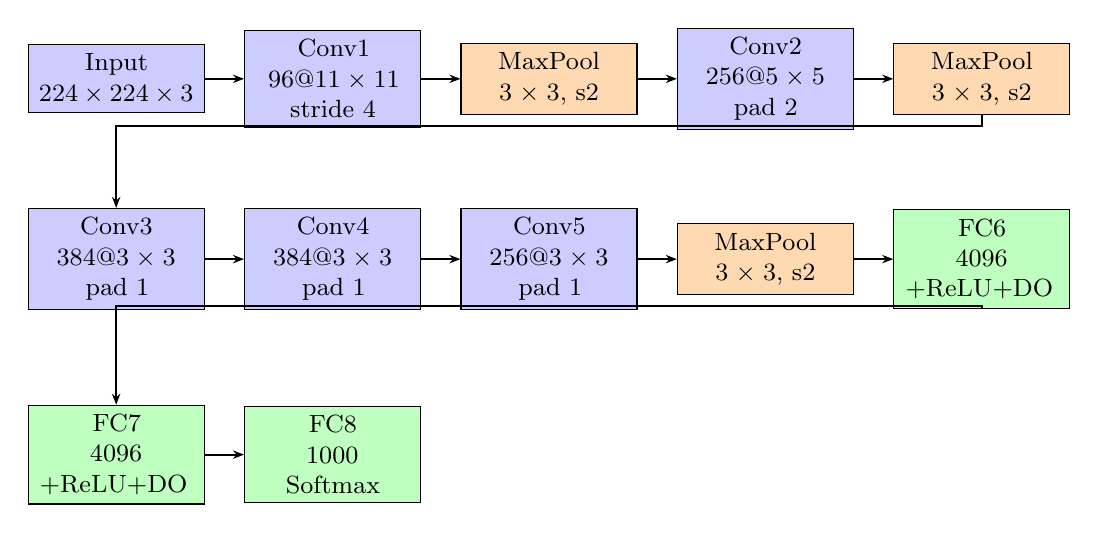
\begin{tikzpicture}[
    node distance=0.6cm and 0.5cm,
    block/.style={rectangle, draw, fill=blue!20, text width=2.0cm, align=center,
                  minimum height=0.7cm, font=\small},
    pool/.style={rectangle, draw, fill=orange!30, text width=2.0cm, align=center,
                 minimum height=0.55cm, font=\small},
    fc/.style={rectangle, draw, fill=green!25, text width=2.0cm, align=center,
               minimum height=0.7cm, font=\small},
    arrow/.style={-{Stealth[length=4pt]}, thick}
  ]
  \node[block] (input) {Input\\$224\times224\times3$};
  \node[block, right=of input] (c1) {Conv1\\96@$11\times11$\\stride 4};
  \node[pool, right=of c1] (p1) {MaxPool\\$3\times3$, s2};
  \node[block, right=of p1] (c2) {Conv2\\256@$5\times5$\\pad 2};
  \node[pool, right=of c2] (p2) {MaxPool\\$3\times3$, s2};
  \node[block, below=1.2cm of input] (c3) {Conv3\\384@$3\times3$\\pad 1};
  \node[block, right=of c3] (c4) {Conv4\\384@$3\times3$\\pad 1};
  \node[block, right=of c4] (c5) {Conv5\\256@$3\times3$\\pad 1};
  \node[pool, right=of c5] (p3) {MaxPool\\$3\times3$, s2};
  \node[fc, right=of p3] (fc6) {FC6\\4096\\+ReLU+DO};
  \node[fc, below=1.2cm of c3] (fc7) {FC7\\4096\\+ReLU+DO};
  \node[fc, right=of fc7] (fc8) {FC8\\1000\\Softmax};

  \draw[arrow] (input) -- (c1);
  \draw[arrow] (c1) -- (p1);
  \draw[arrow] (p1) -- (c2);
  \draw[arrow] (c2) -- (p2);
  \draw[arrow] (p2) -- ++(0,-0.6) -| (c3);
  \draw[arrow] (c3) -- (c4);
  \draw[arrow] (c4) -- (c5);
  \draw[arrow] (c5) -- (p3);
  \draw[arrow] (p3) -- (fc6);
  \draw[arrow] (fc6) -- ++(0,-0.6) -| (fc7);
  \draw[arrow] (fc7) -- (fc8);
\end{tikzpicture}
\caption{AlexNet architecture: five convolutional layers (blue) with max-pooling (orange) followed by three fully-connected layers (green). Dropout is applied at FC6 and FC7.}
\label{fig:alexnet}
\end{figure}

\subsection{Key Innovations}

Four engineering choices enabled AlexNet's success:

\begin{enumerate}[leftmargin=2em]
  \item \textbf{ReLU activation:} $\mathrm{ReLU}(x) = \max(0, x)$ trains several times faster than sigmoid or tanh because it does not saturate in the positive domain and avoids the vanishing gradient problem.
  \begin{equation}
    \mathrm{ReLU}(x) = \max(0,\, x)
    \label{eq:relu}
  \end{equation}
  \item \textbf{Dropout regularization:} With probability $p=0.5$, each neuron in FC6 and FC7 is randomly set to zero during each forward pass of training, preventing co-adaptation of neurons and reducing overfitting.
  \item \textbf{Data augmentation:} Training images are randomly cropped to $224\times224$, horizontally flipped, and perturbed in colour space, artificially increasing the effective dataset size.
  \item \textbf{Multi-GPU training:} The network is split across two NVIDIA GTX 580 GPUs (3 GB memory each), with layers communicating only at selected points. This was essential given the hardware constraints of 2012.
\end{enumerate}

\subsection{ILSVRC Results}

\begin{table}[ht]
\centering
\caption{AlexNet performance on ILSVRC-2010 and ILSVRC-2012 test sets}
\label{tab:alexnet_results}
\begin{tabular}{@{}llcc@{}}
\toprule
Year & Method & Top-1 Error (\%) & Top-5 Error (\%) \\
\midrule
\multirow{3}{*}{2010}
  & Sparse coding (state of the art)   & 47.1 & 28.2 \\
  & SIFT + Fisher vectors (C+FV)        & 45.7 & 25.7 \\
  & AlexNet (1 CNN)                     & 37.5 & 17.0 \\
\midrule
\multirow{2}{*}{2012}
  & Second-best entry (non-DL)          & --   & 26.2 \\
  & AlexNet (ensemble of 7 CNNs)        & --   & 15.3 \\
\bottomrule
\end{tabular}
\end{table}

The gap of $\approx 11$ percentage points in top-5 error at ILSVRC-2012 (from $26.2\%$ to $15.3\%$) was entirely unprecedented in the history of the challenge and immediately attracted worldwide attention to deep learning.

\begin{example}
\textbf{Model ensemble strategy.} The $15.3\%$ top-5 result was achieved by averaging the softmax outputs of seven independently-trained networks: five CNNs with five convolutional layers, one CNN with six convolutional layers, and two CNNs pre-trained on the full ImageNet fall 2011 release. Each network is trained on the same data with slightly different initializations and kernel configurations. Averaging predictions reduces variance and consistently improves accuracy by $1$--$2$ percentage points.
\end{example}

% -------------------------------------------------------
%  4. VGGNET
% -------------------------------------------------------
\section{VGGNet (2014)}
\label{sec:vggnet}

\subsection{Motivation: The Depth Hypothesis}

After the success of AlexNet, researchers asked: \emph{what is the most important architectural dimension -- breadth (number of filters) or depth (number of layers)?} Karen Simonyan and Andrew Zisserman at the Visual Geometry Group (VGG), Oxford, conducted a rigorous investigation: fix all other architectural choices at their simplest values and vary only depth. Their paper, \emph{Very Deep Convolutional Networks for Large-Scale Image Recognition}, appeared at ICLR 2015 \cite{vgg2015}.

\begin{keyinsight}
VGGNet's central contribution is the demonstration that depth using exclusively $3\times3$ convolution filters throughout is the critical factor for achieving strong classification performance. Two stacked $3\times3$ conv layers have the same receptive field as one $5\times5$ layer, but fewer parameters and more non-linearity; three stacked $3\times3$ layers match one $7\times7$ layer, again with fewer parameters.
\end{keyinsight}

\subsection{Receptive Field Analysis}

The effective receptive field equivalence can be verified as follows. Let each $3\times3$ layer apply padding of 1 so that spatial size is preserved. After two such layers, a given output neuron has ``seen'' a $5\times5$ region of the input:
\begin{align}
  r_1 &= 3, \\
  r_2 &= r_1 + (3-1) = 5.
\end{align}
After three layers:
\begin{equation}
  r_3 = 5 + (3-1) = 7.
\end{equation}

Parameter comparison between one $5\times5$ layer and two $3\times3$ layers (both with $C$ channels):
\begin{align}
  \text{Params}(5\times5) &= 5^2 C^2 = 25 C^2, \\
  \text{Params}(2 \times 3\times3) &= 2 \times 3^2 C^2 = 18 C^2.
\end{align}
The two stacked layers use $18/25 = 72\%$ of the parameters and introduce an additional non-linear activation function between them.

\subsection{Architecture Configurations}

VGGNet was evaluated across five depth configurations (A through E). All configurations share:
\begin{itemize}[leftmargin=2em]
  \item Input: $224\times224$ RGB image.
  \item All convolutional filters: $3\times3$, stride 1, padding 1.
  \item Five max-pooling stages: $2\times2$, stride 2.
  \item Three fully-connected layers: FC-4096, FC-4096, FC-1000.
  \item Softmax output for 1000-class classification.
\end{itemize}

The number of convolutional filters doubles with each pooling stage: 64, 128, 256, 512, 512.

\begin{table}[ht]
\centering
\caption{VGGNet configurations A through E with total weight-layer counts and parameter counts}
\label{tab:vgg_configs}
\begin{tabular}{@{}ccccc@{}}
\toprule
Config & Depth (weight layers) & Conv channels & Parameters (M) & Top-5 val.\ error (\%) \\
\midrule
A      & 11 & 64--512 & 133 & 10.4 \\
A-LRN  & 11 & 64--512 & 133 & 10.4 \\
B      & 13 & 64--512 & 133 & 9.9  \\
C      & 16 & 64--512 & 134 & 9.4  \\
D      & 16 & 64--512 & 138 & 8.8  \\
E      & 19 & 64--512 & 144 & 8.7  \\
\bottomrule
\end{tabular}
\end{table}

\noindent Key observation from \cref{tab:vgg_configs}: classification error decreases monotonically as depth increases from 11 to 19 layers, confirming the depth hypothesis. Furthermore, config D (VGG-16) and config E (VGG-19) are the most widely used in practice.

\subsection{Multi-Scale Training}

One important training detail is \emph{multi-scale training}: rather than fixing the training image scale at $S=256$, the scale $S$ is randomly sampled from $[256, 512]$ at each iteration. This acts as a form of scale augmentation, since objects in real images appear at a variety of sizes.

\subsection{ILSVRC Comparison}

\begin{table}[ht]
\centering
\caption{VGGNet vs.\ competing methods on ILSVRC classification (Simonyan \& Zisserman, 2014). Results without external training data only.}
\label{tab:vgg_comparison}
\small
\begin{tabular}{@{}lccc@{}}
\toprule
Method & Top-1 val.\ (\%) & Top-5 val.\ (\%) & Top-5 test (\%) \\
\midrule
VGG (1 net, multi-crop \& dense eval.) -- D  & 24.4 & 7.1  & 7.0 \\
VGG (1 net, multi-crop \& dense eval.) -- E  & 24.7 & 7.5  & 7.3 \\
VGG ILSVRC submission (7 nets, dense)        & 24.7 & 7.5  & 7.1 \\
GoogLeNet (Szegedy et al., 2014) -- 7 nets   & --   & 6.7  & -- \\
MSRA (He et al., 2014) -- 11 nets            & 27.9 & 9.1  & 9.1 \\
Zeiler \& Fergus (2013) -- 6 nets            & 36.0 & 14.7 & 14.8 \\
Zeiler \& Fergus (2013) -- 1 net             & 37.5 & 16.0 & 16.1 \\
OverFeat (Sermanet et al., 2014) -- 1 net    & 34.0 & 13.2 & 13.6 \\
Krizhevsky et al.\ (2012) -- 1 net (AlexNet) & 40.7 & 18.2 & --  \\
\bottomrule
\end{tabular}
\end{table}

\begin{example}
\textbf{Pre-trained model transfer.} A major secondary contribution of VGGNet was demonstrating that features learned on ImageNet transfer well to other visual recognition tasks. Fine-tuning a pre-trained VGG-16 on a target dataset with few samples consistently outperforms training from scratch. This result was instrumental in motivating the large pre-trained model paradigm -- the conceptual precursor to transformer-based foundation models (e.g., BERT, GPT).
\end{example}

\begin{warningbox}
VGGNet's strong performance comes at significant computational cost. VGG-16 has 138 million parameters (compared to AlexNet's 60 million) and requires approximately $15\,\text{GB}$ of memory to train with batch size 256. The three fully-connected layers alone account for the majority of these parameters and most of the inference time. Later architectures (e.g., GoogLeNet, ResNet) achieve better or comparable accuracy with far fewer parameters by eliminating large fully-connected layers.
\end{warningbox}

% -------------------------------------------------------
%  5. RESNET
% -------------------------------------------------------
\section{ResNet (2016)}
\label{sec:resnet}

\subsection{The Degradation Problem}

Following VGGNet's success, the natural question was: \emph{can we keep increasing the depth further?} Experiments with plain networks (no residual connections) revealed a counterintuitive phenomenon: adding more layers beyond a certain threshold actually \emph{increased} both training and test error. This is called the \textbf{degradation problem} and is distinct from overfitting (overfitting would show low training error but high test error).

Kaiming He, Xiangyu Zhang, Shaoqing Ren, and Jian Sun at Microsoft Research addressed this problem in their CVPR 2016 paper \emph{Deep Residual Learning for Image Recognition} \cite{resnet2016}.

\begin{keyinsight}
The degradation problem shows that a 56-layer plain network has \emph{higher training error} than an 18-layer plain network, despite having more capacity. This is not a problem of overfitting -- it is an optimization problem: deep plain networks are simply harder to train. Residual connections solve this by reformulating the learning objective.
\end{keyinsight}

\subsection{Residual Learning Formulation}

In a standard convolutional block, the goal is to learn a mapping $\mathcal{H}(\mathbf{x})$, where $\mathbf{x}$ is the input. ResNet proposes to instead let the stacked non-linear layers fit the \emph{residual function}:
\begin{equation}
  \mathcal{F}(\mathbf{x}) \;=\; \mathcal{H}(\mathbf{x}) - \mathbf{x},
  \label{eq:residual_def}
\end{equation}
so that the desired mapping becomes:
\begin{equation}
  \mathcal{H}(\mathbf{x}) \;=\; \mathcal{F}(\mathbf{x}) + \mathbf{x}.
  \label{eq:residual_mapping}
\end{equation}

This is implemented by a \emph{shortcut connection} (also called a skip connection) that adds the input $\mathbf{x}$ directly to the output of the stacked layers before the final activation:
\begin{equation}
  \mathbf{y} \;=\; \mathcal{F}(\mathbf{x},\, \{W_i\}) + \mathbf{x},
  \label{eq:shortcut}
\end{equation}
where $\{W_i\}$ denotes the weights of the residual branch.

\begin{remark}
If the identity mapping $\mathcal{H}(\mathbf{x}) = \mathbf{x}$ is optimal (i.e., additional layers should not change the representation), it is much easier for the network to push $\mathcal{F}(\mathbf{x}) \to \mathbf{0}$ than to learn the identity function through a stack of non-linear layers. Shortcut connections therefore provide a ``gradient highway'' that allows gradients to flow directly from later layers to earlier layers without passing through non-linearities.
\end{remark}

\subsection{Residual Block Diagram}

\begin{figure}[ht]
\centering
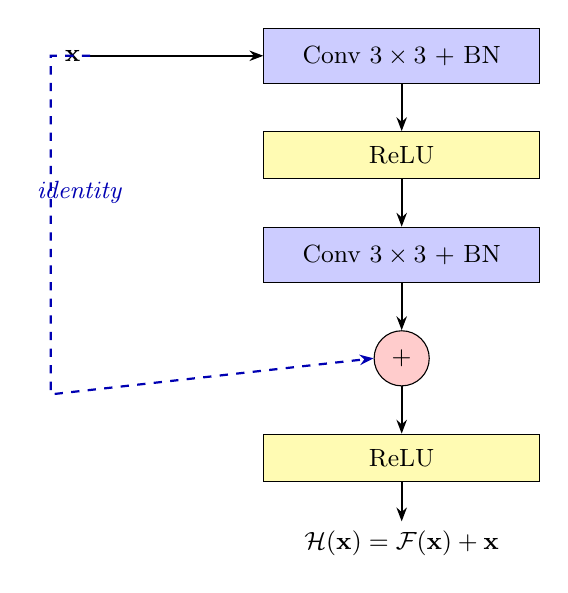
\begin{tikzpicture}[
    node distance=0.8cm,
    conv/.style={rectangle, draw, fill=blue!20, minimum width=3.5cm, minimum height=0.7cm,
                 align=center, font=\small},
    act/.style={rectangle, draw, fill=yellow!30, minimum width=3.5cm, minimum height=0.6cm,
                align=center, font=\small},
    add/.style={circle, draw, fill=red!20, minimum size=0.7cm, font=\small\bfseries},
    arrow/.style={-{Stealth[length=5pt]}, thick}
  ]
  % Main branch
  \node[conv] (conv1) {Conv $3\times3$ + BN};
  \node[act, below=0.6cm of conv1] (relu1) {ReLU};
  \node[conv, below=0.6cm of relu1] (conv2) {Conv $3\times3$ + BN};
  \node[add, below=0.6cm of conv2] (plus) {$+$};
  \node[act, below=0.6cm of plus] (relu2) {ReLU};
  \node[below=0.5cm of relu2, font=\small] (out) {$\mathcal{H}(\mathbf{x}) = \mathcal{F}(\mathbf{x}) + \mathbf{x}$};

  % Skip connection
  \coordinate (skip_start) at ([xshift=-2.5cm]conv1.west);
  \coordinate (skip_end)   at ([xshift=-2.5cm]plus.west);
  \node[left=2.2cm of conv1, font=\small] (x_label) {$\mathbf{x}$};

  \draw[arrow] (x_label) -- (conv1);
  \draw[arrow] (conv1) -- (relu1);
  \draw[arrow] (relu1) -- (conv2);
  \draw[arrow] (conv2) -- (plus);
  \draw[arrow] (plus) -- (relu2);
  \draw[arrow] (relu2) -- (out);

  % Skip path
  \draw[arrow, dashed, blue!70!black, thick]
    (x_label.east) ++(0,0)
    -- ++(-0.5,0)
    -- ++(0,-4.3)
    -- (plus.west);
  \node[above right, font=\small\itshape, blue!70!black] at ([xshift=-3.0cm, yshift=-2.0cm]conv1.west) {identity};
\end{tikzpicture}
\caption{A basic ResNet residual block. The skip connection (dashed blue) adds the input $\mathbf{x}$ directly to the output of the two-layer sub-network, so only the residual $\mathcal{F}(\mathbf{x}) = \mathcal{H}(\mathbf{x}) - \mathbf{x}$ must be learned.}
\label{fig:resblock}
\end{figure}

\subsection{Bottleneck Block}

For deeper variants (ResNet-50/101/152), a \emph{bottleneck} block replaces the basic block to reduce computational cost:
\begin{equation}
  \mathcal{F}(\mathbf{x}) = W_3 \cdot \mathrm{ReLU}(W_2 \cdot \mathrm{ReLU}(W_1 \mathbf{x})),
\end{equation}
where $W_1$ is a $1\times1$ convolution (reducing channels from 256 to 64), $W_2$ is a $3\times3$ convolution, and $W_3$ is a $1\times1$ convolution (expanding back to 256 channels). This $1\times1$--$3\times3$--$1\times1$ pattern processes spatial information at a lower channel dimensionality.

\subsection{Architecture Variants}

\begin{table}[ht]
\centering
\caption{ResNet depth variants: layer composition and top-1 validation error on ILSVRC}
\label{tab:resnet_variants}
\begin{tabular}{@{}lcccc@{}}
\toprule
Variant & Total layers & Block type & Parameters (M) & Top-1 error (\%) \\
\midrule
ResNet-18  & 18  & Basic      & 11.7  & 30.2 \\
ResNet-34  & 34  & Basic      & 21.8  & 26.7 \\
ResNet-50  & 50  & Bottleneck & 25.6  & 24.7 \\
ResNet-101 & 101 & Bottleneck & 44.5  & 23.4 \\
ResNet-152 & 152 & Bottleneck & 60.2  & 23.0 \\
\bottomrule
\end{tabular}
\end{table}

\subsection{Degradation Problem: Quantitative Evidence}

The ResNet paper reported the following comparison on ILSVRC validation:
\begin{itemize}[leftmargin=2em]
  \item Plain-18 top-1 error: $27.94\%$; Plain-34: $28.54\%$ -- \emph{deeper is worse!}
  \item ResNet-18 top-1 error: $27.88\%$; ResNet-34: $25.03\%$ -- \emph{deeper is better.}
\end{itemize}

\subsection{Network Architecture Comparison}

\begin{figure}[ht]
\centering
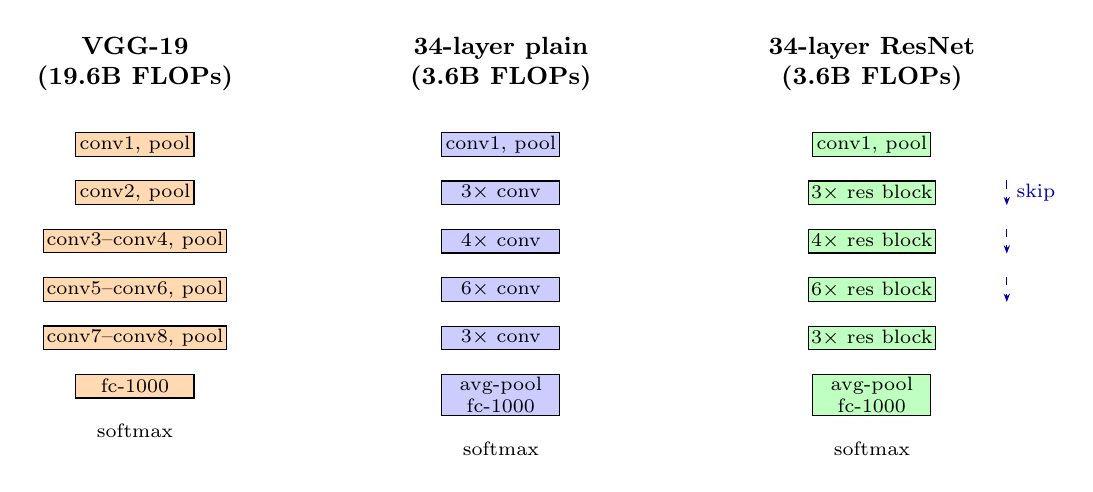
\begin{tikzpicture}[
    node distance=0.3cm and 1.5cm,
    lyr/.style={rectangle, draw, minimum width=1.5cm, minimum height=0.3cm, align=center,
                font=\scriptsize, inner sep=1pt},
    vgg/.style={lyr, fill=orange!30},
    plain/.style={lyr, fill=blue!20},
    res/.style={lyr, fill=green!25},
    title/.style={font=\small\bfseries, align=center},
    arrow/.style={-{Stealth[length=4pt]}, thick}
  ]

  % --- VGG-19 column ---
  \node[title] (vtitle) {VGG-19\\(19.6B FLOPs)};
  \node[vgg, below=0.4cm of vtitle] (v1) {conv1, pool};
  \node[vgg, below=of v1] (v2) {conv2, pool};
  \node[vgg, below=of v2] (v3) {conv3--conv4, pool};
  \node[vgg, below=of v3] (v4) {conv5--conv6, pool};
  \node[vgg, below=of v4] (v5) {conv7--conv8, pool};
  \node[vgg, below=of v5] (v6) {fc-1000};
  \node[below=0.2cm of v6, font=\scriptsize] {softmax};

  % --- 34-layer plain ---
  \node[title, right=2.0cm of vtitle] (ptitle) {34-layer plain\\(3.6B FLOPs)};
  \node[plain, below=0.4cm of ptitle] (p1) {conv1, pool};
  \node[plain, below=of p1] (p2) {$3\times$ conv};
  \node[plain, below=of p2] (p3) {$4\times$ conv};
  \node[plain, below=of p3] (p4) {$6\times$ conv};
  \node[plain, below=of p4] (p5) {$3\times$ conv};
  \node[plain, below=of p5] (p6) {avg-pool\\fc-1000};
  \node[below=0.2cm of p6, font=\scriptsize] {softmax};

  % --- 34-layer residual ---
  \node[title, right=2.0cm of ptitle] (rtitle) {34-layer ResNet\\(3.6B FLOPs)};
  \node[res, below=0.4cm of rtitle] (r1) {conv1, pool};
  \node[res, below=of r1] (r2) {$3\times$ res block};
  \node[res, below=of r2] (r3) {$4\times$ res block};
  \node[res, below=of r3] (r4) {$6\times$ res block};
  \node[res, below=of r4] (r5) {$3\times$ res block};
  \node[res, below=of r5] (r6) {avg-pool\\fc-1000};
  \node[below=0.2cm of r6, font=\scriptsize] {softmax};

  % Skip connection arrows on residual column
  \draw[-{Stealth[length=3pt]}, dashed, blue!70!black]
    ([xshift=0.9cm]r2.north east) -- ([xshift=0.9cm]r2.south east)
    node[midway, right, font=\scriptsize, blue!70!black] {skip};
  \draw[-{Stealth[length=3pt]}, dashed, blue!70!black]
    ([xshift=0.9cm]r3.north east) -- ([xshift=0.9cm]r3.south east);
  \draw[-{Stealth[length=3pt]}, dashed, blue!70!black]
    ([xshift=0.9cm]r4.north east) -- ([xshift=0.9cm]r4.south east);
\end{tikzpicture}
\caption{Side-by-side comparison of VGG-19, 34-layer plain network, and 34-layer ResNet. The residual network uses significantly fewer FLOPs than VGG-19 while achieving better accuracy. Skip connections (dashed blue) bypass pairs of layers in the residual network.}
\label{fig:arch_comparison}
\end{figure}

% -------------------------------------------------------
%  6. ALGORITHMS
% -------------------------------------------------------
\section{Training Algorithms}
\label{sec:algorithms}

\subsection{Standard CNN Training with SGD}

\begin{algorithm}[H]
\caption{Stochastic Gradient Descent Training for CNN Classification}
\label{alg:sgd_cnn}
\SetAlgoLined
\DontPrintSemicolon
\KwIn{Training set $\mathcal{D} = \{(\mathbf{x}_i, y_i)\}_{i=1}^N$, CNN $f_\theta$, learning rate $\eta$, momentum $\mu$, weight decay $\lambda$, epochs $T$}
\KwOut{Optimized parameters $\theta^*$}
Initialize $\theta$ (e.g., He initialization for ReLU networks)\;
$\mathbf{v} \leftarrow \mathbf{0}$ \tcp*{momentum buffer}
\For{$t = 1, 2, \ldots, T$}{
  Shuffle $\mathcal{D}$ into mini-batches $\mathcal{B}_1, \mathcal{B}_2, \ldots$\;
  \For{each mini-batch $\mathcal{B}$}{
    Forward pass: compute logits $\hat{\mathbf{y}} = f_\theta(\mathbf{x})$ for $\mathbf{x} \in \mathcal{B}$\;
    Compute cross-entropy loss:
    $\mathcal{L} = -\dfrac{1}{|\mathcal{B}|}\sum_{(\mathbf{x},y) \in \mathcal{B}} \log \hat{p}_y + \lambda \|\theta\|^2_2$\;
    Backward pass: compute $\mathbf{g} = \nabla_\theta \mathcal{L}$\;
    Update momentum: $\mathbf{v} \leftarrow \mu\,\mathbf{v} + \mathbf{g}$\;
    Update parameters: $\theta \leftarrow \theta - \eta\,\mathbf{v}$\;
  }
  Decay $\eta$ if validation loss plateaus\;
}
\Return $\theta$\;
\end{algorithm}

\subsection{Data Augmentation Strategy}

Both AlexNet and VGGNet use the following data augmentation during training:
\begin{enumerate}[leftmargin=2em]
  \item \textbf{Random crop:} From a rescaled image, randomly extract a $224\times224$ patch.
  \item \textbf{Horizontal flip:} With probability 0.5, flip the patch left-right.
  \item \textbf{Colour jitter (AlexNet only):} Add multiples of the principal components of the RGB pixel values across the training set, sampled from $\mathcal{N}(0, 0.1)$.
  \item \textbf{Multi-scale jitter (VGGNet only):} Randomly sample the rescaling factor $S \in [256, 512]$ before cropping.
\end{enumerate}

During test time, standard practice is to evaluate on 10 crops (4 corners + centre, $\times$ 2 for horizontal flip) and average the softmax outputs.

% -------------------------------------------------------
%  7. COMPARATIVE ANALYSIS
% -------------------------------------------------------
\section{Comparative Analysis and Historical Progression}
\label{sec:comparison}

\subsection{Error Rate Progression on ILSVRC}

The following diagram summarizes the historical progression:

\begin{figure}[ht]
\centering
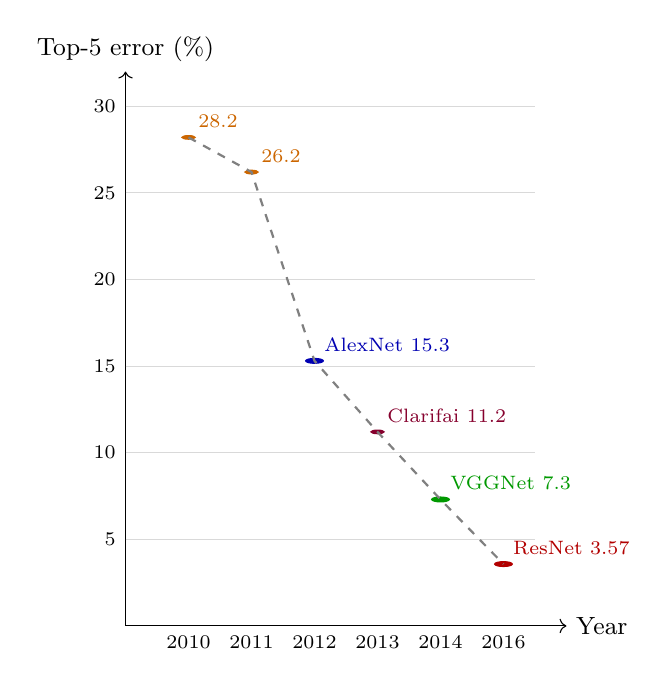
\begin{tikzpicture}
  \begin{scope}[xscale=0.8, yscale=0.22]
    % Axes
    \draw[->] (0,0) -- (7,0) node[right, font=\small] {Year};
    \draw[->] (0,0) -- (0,32) node[above, font=\small] {Top-5 error (\%)};

    % Grid lines
    \foreach \y in {5,10,15,20,25,30} {
      \draw[gray!30] (0,\y) -- (6.5,\y);
      \node[left, font=\scriptsize] at (0,\y) {\y};
    }

    % Year labels
    \foreach \x/\lbl in {1/2010, 2/2011, 3/2012, 4/2013, 5/2014, 6/2016} {
      \node[below, font=\scriptsize] at (\x,0) {\lbl};
    }

    % Prior methods (pre-2012)
    \filldraw[orange!80!black] (1,28.2) circle (3pt) node[above right, font=\scriptsize]{28.2};
    \filldraw[orange!80!black] (2,26.2) circle (3pt) node[above right, font=\scriptsize]{26.2};

    % AlexNet 2012
    \filldraw[blue!70!black] (3,15.3) circle (4pt) node[above right, font=\scriptsize]{AlexNet 15.3};

    % 2013 improvements
    \filldraw[purple!70!black] (4,11.2) circle (3pt) node[above right, font=\scriptsize]{Clarifai 11.2};

    % VGGNet 2014
    \filldraw[green!60!black] (5,7.3) circle (4pt) node[above right, font=\scriptsize]{VGGNet 7.3};

    % ResNet 2016
    \filldraw[red!70!black] (6,3.57) circle (4pt) node[above right, font=\scriptsize]{ResNet 3.57};

    % Connect the dots
    \draw[thick, dashed, gray]
      (1,28.2) -- (2,26.2) -- (3,15.3) -- (4,11.2) -- (5,7.3) -- (6,3.57);
  \end{scope}
\end{tikzpicture}
\caption{Top-5 error rate on ILSVRC from 2010 to 2016. The steep drop from 2011 to 2012 marks the arrival of AlexNet. VGGNet and ResNet continued the trajectory, with ResNet (ensemble) reaching $3.57\%$ -- surpassing estimated human-level performance of approximately $5\%$.}
\label{fig:error_progression}
\end{figure}

\subsection{Architecture Comparison Table}

\begin{table}[ht]
\centering
\caption{Summary comparison of AlexNet, VGGNet, and ResNet architectures}
\label{tab:arch_summary}
\begin{tabular}{@{}lccccc@{}}
\toprule
Architecture & Year & Depth & Params (M) & ILSVRC Top-5 (\%) & Key Innovation \\
\midrule
AlexNet  & 2012 & 8   & 60  & 15.3 & ReLU, Dropout, GPU \\
VGGNet-16 & 2014 & 16  & 138 & 7.3  & Depth with $3\times3$ \\
VGGNet-19 & 2014 & 19  & 144 & 7.0  & Depth with $3\times3$ \\
ResNet-34  & 2016 & 34  & 22  & 7.4  & Residual connections \\
ResNet-50  & 2016 & 50  & 26  & 6.7  & Bottleneck blocks \\
ResNet-152 & 2016 & 152 & 60  & 5.7  & Extreme depth \\
ResNet ens. & 2016 & --  & --  & 3.57 & Ensemble of ResNets \\
\bottomrule
\end{tabular}
\end{table}

\subsection{Design Philosophy Comparison}

Each architecture embodies a distinct design philosophy:

\begin{itemize}[leftmargin=2em]
  \item \textbf{AlexNet:} ``More capacity via moderate depth + many filters + powerful hardware.'' Introduced the toolkit (ReLU, Dropout, data augmentation, GPU) that all subsequent architectures rely on.
  \item \textbf{VGGNet:} ``Depth with small filters is the key factor.'' Showed that a uniform $3\times3$ filter strategy, pushed to 16--19 layers, outperforms shallower architectures with larger filters and more parameters.
  \item \textbf{ResNet:} ``Residual learning solves the optimization problem of very deep networks.'' The key insight is not just depth but \emph{trainable depth}: skip connections make it possible to reliably optimize networks with hundreds of layers.
\end{itemize}

\begin{keyinsight}
The transition from AlexNet to VGGNet to ResNet reflects a general principle in deep learning: \emph{depth is more important than breadth for representational power}, but only when the optimization problem associated with deep networks is properly addressed. ResNet's residual formulation is the solution to that optimization problem.
\end{keyinsight}

% -------------------------------------------------------
%  8. MATHEMATICAL DETAILS
% -------------------------------------------------------
\section{Mathematical Details}
\label{sec:math}

\subsection{Convolutional Layer Forward Pass}

Given an input feature map $\mathbf{X} \in \mathbb{R}^{H \times W \times C_{\text{in}}}$ and a filter bank $\mathbf{W} \in \mathbb{R}^{K \times K \times C_{\text{in}} \times C_{\text{out}}}$ with bias $\mathbf{b} \in \mathbb{R}^{C_{\text{out}}}$, the output at spatial location $(i,j)$ for output channel $k$ is:
\begin{equation}
  \mathbf{Y}_{i,j,k} = b_k + \sum_{c=1}^{C_{\text{in}}} \sum_{p=0}^{K-1} \sum_{q=0}^{K-1}
    \mathbf{W}_{p,q,c,k} \cdot \mathbf{X}_{i\cdot s + p,\, j\cdot s + q,\, c},
  \label{eq:conv}
\end{equation}
where $s$ is the stride.

\subsection{Batch Normalization}

ResNet layers include Batch Normalization (BN) after each convolution and before each activation:
\begin{align}
  \hat{x}_i &= \frac{x_i - \mu_\mathcal{B}}{\sqrt{\sigma^2_\mathcal{B} + \epsilon}},
  \label{eq:bn_norm}\\
  y_i &= \gamma \hat{x}_i + \beta,
  \label{eq:bn_scale}
\end{align}
where $\mu_\mathcal{B}$ and $\sigma^2_\mathcal{B}$ are the mini-batch mean and variance, and $\gamma$, $\beta$ are learned scale and shift parameters. BN accelerates training by reducing internal covariate shift and allows higher learning rates.

\subsection{Cross-Entropy Loss with Softmax}

For a $C$-class classification problem, the model outputs a logit vector $\mathbf{z} \in \mathbb{R}^C$. The softmax function converts logits to probabilities:
\begin{equation}
  \hat{p}_c = \frac{e^{z_c}}{\sum_{j=1}^{C} e^{z_j}},
  \qquad c = 1, \ldots, C.
  \label{eq:softmax}
\end{equation}
The cross-entropy loss for a batch of $N$ samples is:
\begin{equation}
  \mathcal{L} = -\frac{1}{N} \sum_{i=1}^{N} \log \hat{p}_{y_i},
  \label{eq:ce_loss}
\end{equation}
where $y_i$ is the ground-truth class label for sample $i$.

\subsection{L2 Regularization and Effective Learning}

All three architectures use L2 weight decay (equivalent to a Gaussian prior on weights):
\begin{equation}
  \mathcal{L}_{\text{reg}} = \mathcal{L}_{\text{CE}} + \frac{\lambda}{2} \|\theta\|^2_2,
  \label{eq:l2_reg}
\end{equation}
where $\lambda$ is the weight decay coefficient (typically $5\times10^{-4}$ for AlexNet and VGGNet, $10^{-4}$ for ResNet).

% -------------------------------------------------------
%  9. SUMMARY
% -------------------------------------------------------
\section{Summary}
\label{sec:summary}

Session 14 traced the arc of CNN architecture development from the AlexNet breakthrough of 2012 to the ResNet ensemble result of 2016 -- a trajectory that reduced ILSVRC top-5 error from $26.2\%$ to $3.57\%$ in four years.

\paragraph{AlexNet (NIPS 2012).}
Five convolutional layers and three fully-connected layers; 60 million parameters; trained on two GPUs. Key innovations: ReLU activations for faster training, Dropout for regularization, and data augmentation. Achieved $15.3\%$ top-5 error at ILSVRC-2012, an $11$ percentage point improvement over the non-deep-learning runner-up.

\paragraph{VGGNet (ICLR 2015).}
Depth-first exploration using exclusively $3\times3$ filters. Configurations from 11 to 19 weight layers, all with 64--512 filters doubling after each pooling. Achieved $7.3\%$ top-5 test error (VGG-16) and $7.0\%$ (VGG-19) at ILSVRC-2014. Introduced the concept of deep, pre-trained CNN features that generalize to other tasks -- a precursor to transfer learning.

\paragraph{ResNet (CVPR 2016).}
Introduced residual (skip) connections to address the \emph{degradation problem}: plain networks with more than $\sim$20 layers exhibited \emph{higher} training error than shallower networks. The residual formulation $\mathcal{H}(\mathbf{x}) = \mathcal{F}(\mathbf{x}) + \mathbf{x}$ made it possible to train networks with 34, 50, 101, and 152 layers, achieving $5.7\%$ top-5 error with ResNet-152 and $3.57\%$ with an ensemble -- surpassing human-level performance on ILSVRC for the first time.

\medskip

These three architectures established the foundational design patterns of modern deep learning: ReLU activations, batch normalization, residual connections, and depth-first design. They remain the backbone of countless production systems and the starting point for new research across vision, speech, and beyond.

\begin{keyinsight}
The Instructor's recommendation: read all three original papers -- Krizhevsky et al.\ (2012), Simonyan \& Zisserman (2014), and He et al.\ (2016) -- not only for their technical content but for the clarity of their experimental methodology and the impact of their results on the trajectory of the entire field.
\end{keyinsight}

% -------------------------------------------------------
%  APPENDIX A: PRACTICAL NOTES AND TRANSFER LEARNING
% -------------------------------------------------------
\section{Practical Notes: Transfer Learning and Pre-trained Models}
\label{sec:transfer}

\subsection{The Pre-trained Model Paradigm}

One of the most practically significant outcomes of the VGGNet and ResNet era was the establishment of the \emph{pre-trained model} paradigm. The core idea is:

\begin{enumerate}[leftmargin=2em]
  \item Train a deep CNN on a very large labelled dataset (e.g., ImageNet with 1.2 million images).
  \item Use the learned weights as a starting point (``initialization'') for a related task where labelled data is scarce.
  \item \emph{Fine-tune} some or all of the network's weights on the target task.
\end{enumerate}

This approach is justified by the observation that the lower layers of a deep CNN learn general-purpose visual features (edges, textures, colour blobs) that are broadly useful across many visual tasks, while only the upper layers specialize to the specific classes in the training dataset.

\begin{example}
\textbf{Medical image analysis using VGG-16 transfer learning.} Suppose a hospital has 5000 labelled chest X-rays (``normal'' vs.\ ``pneumonia''). Training a deep CNN from scratch on 5000 images is likely to overfit. Instead:
\begin{enumerate}[leftmargin=2em]
  \item Download VGG-16 pre-trained on ImageNet.
  \item Replace the final FC-1000 layer with FC-2 (two output classes).
  \item Freeze weights in Conv1--Conv3 (general low-level features).
  \item Fine-tune Conv4, Conv5, and the new FC layers at a low learning rate ($10^{-5}$).
\end{enumerate}
This typically achieves accuracy 10--15\% higher than training from scratch, despite the ImageNet pre-training data containing no medical images.
\end{example}

\subsection{Feature Extraction vs.\ Fine-Tuning}

Two standard strategies exist for applying pre-trained models:

\begin{table}[ht]
\centering
\caption{Comparison of feature extraction and fine-tuning strategies for transfer learning}
\label{tab:transfer_strategies}
\begin{tabular}{@{}lcccc@{}}
\toprule
Strategy & Frozen layers & Trainable layers & Data required & Computation \\
\midrule
Feature extraction & All conv layers & FC layers only & Very small & Low \\
Partial fine-tuning & Conv1--Conv3 & Conv4+, FC & Small--medium & Medium \\
Full fine-tuning & None & All layers & Large & High \\
\bottomrule
\end{tabular}
\end{table}

\subsection{Why Residual Networks Changed Everything}

The success of ResNet had a broader impact beyond ILSVRC. The residual connection principle was quickly adopted in:

\begin{itemize}[leftmargin=2em]
  \item \textbf{Object detection:} Faster R-CNN with ResNet backbone replaced VGG.
  \item \textbf{Semantic segmentation:} DeepLab and FCN architectures adopted residual backbones.
  \item \textbf{Natural language processing:} The Transformer architecture (2017) uses residual connections in both the encoder and decoder, explicitly crediting the ResNet design.
  \item \textbf{Speech processing:} Deep residual networks for acoustic modeling followed the ResNet paper.
\end{itemize}

\begin{remark}
The instructor noted that VGGNet's demonstration of powerful pre-trained features directly motivated the development of transformer-based large pre-trained models (BERT, GPT, etc.\ for NLP). The question ``can we have an equivalent of VGGNet/ResNet for sequence data?'' led to the proposal and rapid adoption of the Transformer architecture.
\end{remark}

% -------------------------------------------------------
%  APPENDIX B: GRADIENT FLOW IN DEEP NETWORKS
% -------------------------------------------------------
\section{Gradient Flow Analysis}
\label{sec:gradient_flow}

\subsection{Vanishing Gradients in Plain Networks}

For a plain $L$-layer network without skip connections, the gradient of the loss $\mathcal{L}$ with respect to weights at layer $\ell$ is:
\begin{equation}
  \frac{\partial \mathcal{L}}{\partial W_\ell}
  = \frac{\partial \mathcal{L}}{\partial \mathbf{z}_L}
    \cdot \prod_{k=\ell+1}^{L} \frac{\partial \mathbf{z}_k}{\partial \mathbf{z}_{k-1}}
    \cdot \frac{\partial \mathbf{z}_\ell}{\partial W_\ell},
  \label{eq:chain_rule}
\end{equation}
where $\mathbf{z}_k$ is the pre-activation at layer $k$. Each Jacobian $\frac{\partial \mathbf{z}_k}{\partial \mathbf{z}_{k-1}}$ depends on the weight matrix and the activation derivative. For ReLU activations and poorly conditioned weight matrices, these Jacobians have singular values that are typically $< 1$, so the product in \cref{eq:chain_rule} decays exponentially with depth, causing \emph{vanishing gradients}.

\subsection{Gradient Flow Through Skip Connections}

For a residual block $\mathbf{y} = \mathcal{F}(\mathbf{x}) + \mathbf{x}$, the gradient with respect to the input $\mathbf{x}$ is:
\begin{equation}
  \frac{\partial \mathcal{L}}{\partial \mathbf{x}}
  = \frac{\partial \mathcal{L}}{\partial \mathbf{y}}
    \cdot \left(\frac{\partial \mathcal{F}(\mathbf{x})}{\partial \mathbf{x}} + \mathbf{I}\right),
  \label{eq:resgrad}
\end{equation}
where $\mathbf{I}$ is the identity matrix. The identity term guarantees that even if $\frac{\partial \mathcal{F}}{\partial \mathbf{x}} \approx \mathbf{0}$ (the residual branch contributes little to learning), the gradient $\frac{\partial \mathcal{L}}{\partial \mathbf{x}}$ is still approximately $\frac{\partial \mathcal{L}}{\partial \mathbf{y}}$ -- not attenuated. This is the mathematical reason that residual networks can be trained successfully to arbitrary depth.

\begin{theorem}[Gradient Propagation Bound for ResNets]
\label{thm:resnet_grad}
Consider a residual network with $L$ blocks, each satisfying $\mathbf{y}_\ell = \mathcal{F}_\ell(\mathbf{x}_\ell) + \mathbf{x}_\ell$. Expanding the chain rule recursively, the gradient at any intermediate layer $\ell$ contains a direct sum-path from the output:
\begin{equation}
  \frac{\partial \mathcal{L}}{\partial \mathbf{x}_\ell}
  = \frac{\partial \mathcal{L}}{\partial \mathbf{x}_L}
    \cdot \left(\mathbf{I} + \sum_{k=\ell}^{L-1} \prod_{j=k}^{L-1}
      \frac{\partial \mathcal{F}_j}{\partial \mathbf{x}_j}\right).
  \label{eq:resnet_grad_bound}
\end{equation}
The identity term $\mathbf{I}$ ensures that the gradient never vanishes to zero, regardless of the depth $L$ or the magnitudes of the residual Jacobians.
\end{theorem}

\subsection{He Initialization}

To complement residual learning, He et al.\ proposed a weight initialization scheme designed for ReLU networks:
\begin{equation}
  W \sim \mathcal{N}\!\left(0,\, \frac{2}{n_{\text{in}}}\right),
  \label{eq:he_init}
\end{equation}
where $n_{\text{in}}$ is the fan-in (number of input units to the layer). This initialization preserves the variance of activations through the forward pass and of gradients through the backward pass for ReLU networks, enabling stable training from the very start.

\begin{warningbox}
Using the Glorot/Xavier initialization (designed for tanh/sigmoid) with ReLU networks causes activations to diminish in deep networks because it does not account for the factor of $1/2$ introduced by the ReLU non-linearity (which zeros out half of all activations on average). He initialization corrects for this by doubling the variance.
\end{warningbox}

% -------------------------------------------------------
%  APPENDIX C: REVIEW QUESTIONS
% -------------------------------------------------------
\section{Review Questions}
\label{sec:review}

The following questions test understanding of the key concepts from Session 14.

\begin{enumerate}[leftmargin=2em, label=\textbf{Q\arabic*.}]

  \item \textbf{Top-$k$ error.}
  A model outputs the following class probabilities for a test image with true label ``cat'' (class 3):
  \[
    [\underbrace{0.4}_{\text{class 1}},\; \underbrace{0.3}_{\text{class 2}},\;
     \underbrace{0.15}_{\text{class 3}},\; \underbrace{0.1}_{\text{class 4}},\;
     \underbrace{0.05}_{\text{class 5}}]
  \]
  Compute the top-1 error and top-5 error for this prediction.

  \item \textbf{Receptive field.}
  Show that three stacked $3\times3$ convolutional layers (stride 1, padding 1) have the same receptive field as one $7\times7$ layer. How many parameters does each require for $C=128$ input and output channels?

  \item \textbf{Degradation problem.}
  A plain 56-layer network has higher training error than an 18-layer network on the same dataset. Is this evidence of: (a) overfitting, (b) underfitting, or (c) an optimization problem? Justify your answer.

  \item \textbf{Residual learning.}
  Suppose a residual block learns $\mathcal{F}(\mathbf{x}) = \mathbf{0}$. What does the block output? What does this imply about the ability of residual networks to represent shallower functions?

  \item \textbf{Transfer learning.}
  You have a dataset of 10,000 satellite images labelled as ``urban'' or ``non-urban''. Would you prefer to: (a) train a ResNet-50 from scratch, (b) use ResNet-50 features with a linear classifier, or (c) fine-tune the top half of a pre-trained ResNet-50? Justify your choice.

  \item \textbf{Parameter count.}
  AlexNet's fully-connected layers (FC6, FC7, FC8) contain approximately how many of the 60 million total parameters? (Hint: FC6 input is $6\times6\times256=9216$ units; FC6 has 4096 neurons; FC7 has 4096 neurons; FC8 has 1000 neurons.)

\end{enumerate}

% -------------------------------------------------------
%  APPENDIX D: VGGNET DEPTH CONFIGURATIONS -- DETAILED
% -------------------------------------------------------
\section{VGGNet Depth Configurations in Detail}
\label{sec:vgg_detail}

\subsection{Filter Progression and Spatial Dimensions}

The following traces the spatial dimensions and filter counts for VGG-16 (configuration D):

\begin{table}[ht]
\centering
\caption{VGG-16 (configuration D) layer-by-layer spatial and channel dimensions}
\label{tab:vgg16_detail}
\small
\begin{tabular}{@{}clccc@{}}
\toprule
Stage & Layers & Input size & Filters & Output size \\
\midrule
1 & Conv3-64, Conv3-64, MaxPool & $224\times224\times3$   & 64  & $112\times112\times64$ \\
2 & Conv3-128, Conv3-128, MaxPool & $112\times112\times64$  & 128 & $56\times56\times128$ \\
3 & Conv3-256 $\times3$, MaxPool & $56\times56\times128$   & 256 & $28\times28\times256$ \\
4 & Conv3-512 $\times3$, MaxPool & $28\times28\times256$   & 512 & $14\times14\times512$ \\
5 & Conv3-512 $\times3$, MaxPool & $14\times14\times512$   & 512 & $7\times7\times512$ \\
6 & FC-4096, FC-4096, FC-1000    & $7\times7\times512=25088$ & -- & 1000 \\
\bottomrule
\end{tabular}
\end{table}

\subsection{Why 1$\times$1 Convolutions Appear in Config C}

Configuration C introduces $1\times1$ convolution layers in addition to $3\times3$ layers. A $1\times1$ convolution applies a linear transformation to the channel dimension at each spatial location independently:
\begin{equation}
  \mathbf{Y}_{i,j,k} = \sum_{c=1}^{C_{\text{in}}} W_{c,k} \cdot \mathbf{X}_{i,j,c}.
  \label{eq:1x1conv}
\end{equation}
This is equivalent to a fully-connected layer applied channel-wise, allowing the network to increase non-linearity (by adding an extra ReLU) without increasing the spatial receptive field. The VGGNet paper found that config D (no $1\times1$ convolutions) outperformed config C (with $1\times1$ convolutions) at the same depth, confirming that spatial context captured by $3\times3$ filters is more important than additional non-linearity from $1\times1$ filters.

\subsection{Multi-Scale Testing}

At test time, VGGNet applies the network at multiple scales $Q \in \{S-32, S, S+32\}$ (where $S$ is the training scale) and averages the resulting class score maps. This is called \emph{dense evaluation} and differs from the simpler multi-crop evaluation used by AlexNet. Dense evaluation converts FC layers to $1\times1$ convolutional layers, allowing the network to process images of arbitrary size and produce a spatial score map rather than a single vector.

\begin{example}
\textbf{Dense vs.\ multi-crop evaluation.}
For a test image of size $384\times384$ (with $S=256$ training scale):
\begin{itemize}[leftmargin=2em]
  \item \emph{Multi-crop:} Extract 10 crops of size $224\times224$, classify each, average.
  \item \emph{Dense:} Convert FC to $1\times1$ conv, apply to full $384\times384$ image. The network outputs a $6\times6\times1000$ score map. Average over the $36$ spatial positions.
\end{itemize}
Dense evaluation is more computationally efficient than multi-crop because computations are shared between overlapping receptive fields.
\end{example}

% -------------------------------------------------------
%  APPENDIX E: RESNET BOTTLENECK AND IDENTITY SHORTCUTS
% -------------------------------------------------------
\section{ResNet Bottleneck Blocks and Projection Shortcuts}
\label{sec:resnet_bottleneck}

\subsection{When Skip Connections Need Projection}

In the basic ResNet formulation, the skip connection performs an identity mapping: $\mathbf{y} = \mathcal{F}(\mathbf{x}) + \mathbf{x}$. This requires $\mathbf{x}$ and $\mathcal{F}(\mathbf{x})$ to have the same dimensions. When the number of channels or spatial dimensions change (e.g., when transitioning between stages), a \emph{projection shortcut} is used:
\begin{equation}
  \mathbf{y} = \mathcal{F}(\mathbf{x},\, \{W_i\}) + W_s \mathbf{x},
  \label{eq:projection_shortcut}
\end{equation}
where $W_s$ is a $1\times1$ convolutional projection that matches dimensions. In ResNet-50/101/152, projection shortcuts are used only when dimensions change; all other skip connections remain identity mappings.

\subsection{Bottleneck Parameter Count}

For a bottleneck block with $d=256$ input/output channels and $d'=64$ bottleneck channels:
\begin{align}
  \text{Params}(\text{bottleneck}) &= d \cdot d' \cdot 1^2 + d' \cdot d' \cdot 3^2 + d' \cdot d \cdot 1^2 \notag \\
  &= 256 \cdot 64 + 64 \cdot 64 \cdot 9 + 64 \cdot 256 \notag \\
  &= 16384 + 36864 + 16384 = 69632.
  \label{eq:bottleneck_params}
\end{align}
For comparison, a basic block with two $3\times3$ convolutions at $d=256$ channels requires:
\begin{equation}
  \text{Params}(\text{basic}) = 2 \times 256 \times 256 \times 9 = 1{,}179{,}648.
  \label{eq:basic_params}
\end{equation}
The bottleneck reduces parameter count by a factor of approximately 17, enabling much greater depth at the same computational budget.

\begin{keyinsight}
The bottleneck design principle -- compress to a lower-dimensional representation, process spatially, then expand -- recurs throughout modern deep learning: it appears in MobileNet's depthwise separable convolutions, in the Transformer's feed-forward sublayer ($d_{\text{model}} \to 4 d_{\text{model}} \to d_{\text{model}}$), and in the inverted residual blocks of MobileNetV2.
\end{keyinsight}

% -------------------------------------------------------
%  REFERENCES
% -------------------------------------------------------
\begin{thebibliography}{9}

\bibitem{alexnet2012}
Alex Krizhevsky, Ilya Sutskever, and Geoffrey E.\ Hinton.
\newblock ImageNet Classification with Deep Convolutional Neural Networks.
\newblock In \emph{Advances in Neural Information Processing Systems (NIPS)}, 2012.

\bibitem{vgg2015}
Karen Simonyan and Andrew Zisserman.
\newblock Very Deep Convolutional Networks for Large-Scale Image Recognition.
\newblock In \emph{International Conference on Learning Representations (ICLR)}, 2015.

\bibitem{resnet2016}
Kaiming He, Xiangyu Zhang, Shaoqing Ren, and Jian Sun.
\newblock Deep Residual Learning for Image Recognition.
\newblock In \emph{Proceedings of the IEEE Conference on Computer Vision and Pattern Recognition (CVPR)}, 2016.

\bibitem{zeiler2013}
Matthew D.\ Zeiler and Rob Fergus.
\newblock Visualizing and Understanding Convolutional Networks.
\newblock In \emph{European Conference on Computer Vision (ECCV)}, 2014.

\bibitem{overfeat2014}
Pierre Sermanet, David Eigen, Xiang Zhang, Michael Mathieu, Rob Fergus, and Yann LeCun.
\newblock OverFeat: Integrated Recognition, Localization and Detection using Convolutional Networks.
\newblock In \emph{ICLR}, 2014.

\end{thebibliography}

\clearpage

%% ============================================================
%% Session 15: CNN Parameter Calculations, Output Size Formulae, and L2 Regularisation
%% ============================================================
\part{Session 15: CNN Parameter Calculations, Output Size Formulae, and L2 Regularisation}

% ════════════════════════════════════════════════════════════════════════════
%  TITLE PAGE
% ════════════════════════════════════════════════════════════════════════════
\begin{titlepage}
  \centering
  \vspace*{2cm}
  {\LARGE\bfseries Deep Learning with PyTorch\\[0.4em]
   \large IIIT Dharwad --- Course Lecture Notes\par}
  \vspace{1.5cm}
  \rule{\linewidth}{0.5pt}\\[0.4em]
  {\huge\bfseries Session 15\\[0.3em]
   \Large CNN Parameter Calculations,\\
   Output Size Formulae, and\\
   L2 Regularisation\par}
  \rule{\linewidth}{0.5pt}
  \vspace{1.5cm}
  \begin{tabular}{ll}
    \textbf{Session Number:} & 15 \\[4pt]
    \textbf{Topic:}          & CNN Exam Q\&A --- Parameter Counting, \\
                             & Convolution Output Sizes, L2 Regularisation \\[4pt]
    \textbf{Slide Deck:}     & \texttt{08\_PyTorchDL\_RNN} (transition deck) \\[4pt]
    \textbf{Instructors:}    & Prof.\ S.~R.~M.\ Prasanna \&
                               Dr.\ Sunil Saumya \\[4pt]
    \textbf{Institution:}    & IIIT Dharwad \\[4pt]
    \textbf{Date:}           & Academic Year 2024--25 \\[4pt]
    \textbf{Video:}          & \url{https://vimeo.com/1153110691} \\
  \end{tabular}
  \vfill
  {\small These notes are compiled from the session transcript and visual
   extractions. Session 15 was conducted as a student-driven Q\&A and
   doubt-clearing session covering CNN parameter calculations, convolution
   output size formulae, and L2 regularisation, serving as consolidation
   before the transition to Recurrent Neural Networks.}
\end{titlepage}

% ════════════════════════════════════════════════════════════════════════════
%  TABLE OF CONTENTS
% ════════════════════════════════════════════════════════════════════════════

\newpage

% ════════════════════════════════════════════════════════════════════════════
\section{Introduction}
\label{sec:intro}
% ════════════════════════════════════════════════════════════════════════════

Session 15 of the \emph{Deep Learning with PyTorch} course at IIIT Dharwad
was conducted as an interactive Q\&A and doubt-clearing class rather than a
conventional lecture. No slide deck was screen-shared; instead, students
raised questions on camera and the instructors---Prof.\ S.~R.~M.\ Prasanna
and Dr.\ Sunil Saumya---clarified key concepts from the preceding CNN
sessions in real time.

The session centred on three tightly connected topics:

\begin{enumerate}[label=\textbf{(\arabic*)}]
  \item \textbf{Convolutional layer parameter counting}: How to derive the
        exact number of trainable weights and biases in a single
        \texttt{Conv2d} layer, and why the count is dramatically smaller
        than an equivalent fully-connected layer.
  \item \textbf{Output spatial size with padding}: The general formula
        $\floor{(N - F + 2P)/S} + 1$ and the three most common padding
        regimes encountered in practice.
  \item \textbf{L2 regularisation (weight decay)}: The relationship between
        the mathematical penalty $\lambda \sum_i w_i^2$, the gradient update
        rule, and PyTorch's \texttt{weight\_decay} argument in
        \texttt{optim.Adam} and \texttt{optim.SGD}.
\end{enumerate}

Together, these topics represent core ``nuts and bolts'' knowledge that
every practitioner must be comfortable with before moving to more complex
architectures. \Cref{sec:background} reviews the CNN building blocks
required as prerequisites. \Cref{sec:param_count} treats parameter counting
in depth. \Cref{sec:output_size} covers output size formulae.
\Cref{sec:l2reg} develops L2 regularisation theory and its PyTorch
implementation. \Cref{sec:comparison} places these ideas in a broader
comparative context. \Cref{sec:conclusion} summarises the session and
previews the transition to Recurrent Neural Networks.

\begin{keyinsight}
This session bridges the CNN module and the forthcoming RNN module. Mastery
of parameter counting and regularisation is prerequisite for reasoning about
model capacity, computational cost, and generalisation in any architecture.
\end{keyinsight}

% ════════════════════════════════════════════════════════════════════════════
\section{Background and Prerequisites}
\label{sec:background}
% ════════════════════════════════════════════════════════════════════════════

\subsection{Convolutional Neural Network Recap}

A Convolutional Neural Network (CNN) processes grid-structured data (images,
feature maps) through a sequence of learnable linear filters followed by
non-linear activations and spatial pooling. The key inductive biases
exploited are \emph{local connectivity} and \emph{weight sharing}.

\begin{definition}[Convolutional Layer]
\label{def:conv_layer}
A convolutional layer with $\Cout$ filters, each of spatial size $F \times F$
applied to an input tensor of spatial size $N \times N$ with $\Cin$ channels
produces an output tensor of shape
\[
  \Cout \;\times\;
  \underbrace{\floor{\tfrac{N - F + 2P}{S}} + 1}_{H_{\mathrm{out}}}
  \;\times\;
  \underbrace{\floor{\tfrac{N - F + 2P}{S}} + 1}_{W_{\mathrm{out}}}
\]
where $P$ is zero-padding (per side) and $S$ is the stride.
\end{definition}

\subsection{Notation Summary}

\Cref{tab:notation} collects the symbols used throughout these notes.

\begin{table}[ht]
  \centering
  \caption{Notation used in Session 15 notes.}
  \label{tab:notation}
  \begin{tabular}{@{}cll@{}}
    \toprule
    Symbol & Meaning & Typical values \\
    \midrule
    $N$     & Input spatial dimension (height or width) & 7, 28, 224 \\
    $F$     & Filter/kernel spatial size                & 1, 3, 5    \\
    $\Cin$  & Number of input channels                  & 1, 3, 64, 128 \\
    $\Cout$ & Number of output filters                  & 32, 64, 256 \\
    $P$     & Zero-padding (applied each side)          & 0, 1, 2 \\
    $S$     & Stride                                    & 1, 2 \\
    $\lambda$ & L2 regularisation coefficient           & $10^{-4}$--$10^{-2}$ \\
    $\eta$  & Learning rate                             & $10^{-3}$--$10^{-1}$ \\
    \bottomrule
  \end{tabular}
\end{table}

\subsection{PyTorch \texttt{Conv2d} API}

In PyTorch the primary interface is:

\begin{verbatim}
torch.nn.Conv2d(in_channels, out_channels, kernel_size,
                stride=1, padding=0, bias=True)
\end{verbatim}

The argument \texttt{bias=True} (default) adds one learnable scalar bias per
output filter. This single flag controls whether bias terms appear in the
parameter count.

\begin{remark}
\label{rem:bias_default}
Because \texttt{bias=True} is the default, exam questions that do not
explicitly state ``no bias'' should be answered \emph{with} bias terms
included. During the session, the instructors confirmed this interpretation.
\end{remark}

% ════════════════════════════════════════════════════════════════════════════
\section{Convolutional Layer Parameter Counting}
\label{sec:param_count}
% ════════════════════════════════════════════════════════════════════════════

\subsection{Derivation of the Parameter Formula}

Each output filter is a 3-D weight tensor of shape $F \times F \times \Cin$
plus one scalar bias. There are $\Cout$ such filters. The total number of
trainable parameters is therefore

\begin{equation}
  \label{eq:param_formula}
  \boxed{P_{\mathrm{conv}} = \bigl(F \times F \times \Cin + 1\bigr) \times \Cout}
\end{equation}

\noindent
where the $+1$ accounts for the bias term. If \texttt{bias=False} is set,
the formula reduces to $(F^2 \cdot \Cin) \cdot \Cout$.

\begin{keyinsight}
The parameter count of a \texttt{Conv2d} layer is \emph{independent of the
input spatial size} $N$. Doubling the input resolution does \emph{not} change
the number of learnable parameters---it only changes the number of times each
filter is applied (the number of output locations). This is the essence of
\textbf{weight sharing}.
\end{keyinsight}

\subsection{Worked Example: 64 Filters, 3\texttimes3, 128 Input Channels}

The exam question that arose during Session 15 was:

\begin{quote}
\itshape
``A convolutional layer has 64 filters, a kernel size of $3 \times 3$, and
128 input channels. How many trainable parameters does it have?''
\end{quote}

Applying \cref{eq:param_formula} with $F = 3$, $\Cin = 128$, $\Cout = 64$:

\begin{align}
  P_{\mathrm{conv}}
    &= \bigl(3 \times 3 \times 128 + 1\bigr) \times 64 \notag \\
    &= \bigl(1152 + 1\bigr) \times 64 \notag \\
    &= 1153 \times 64 \notag \\
    &= \mathbf{73{,}792} \label{eq:example_count}
\end{align}

\noindent
\textbf{Breakdown:}
\begin{itemize}[noitemsep]
  \item Weight parameters: $3 \times 3 \times 128 \times 64 = 73{,}728$
  \item Bias parameters: $64$ (one per output filter)
  \item \textbf{Total: $73{,}792$}
\end{itemize}

\begin{example}[title=Step-by-step parameter count]
\textbf{Given:} \texttt{nn.Conv2d(128, 64, kernel\_size=3)}

\medskip
\begin{tabular}{@{}lrl@{}}
  \toprule
  Component & Calculation & Value \\
  \midrule
  Weights per filter & $3 \times 3 \times 128$ & 1,152 \\
  Filters            & 64                      & --- \\
  Total weights      & $1152 \times 64$        & 73,728 \\
  Bias terms         & $1 \times 64$           & 64 \\
  \midrule
  \textbf{Grand total} & $73728 + 64$ & \textbf{73,792} \\
  \bottomrule
\end{tabular}
\end{example}

\subsection{Parameter Counting TikZ Diagram}
\label{subsec:param_diagram}

\Cref{fig:param_count} illustrates the weight-sharing structure that leads
to \cref{eq:param_formula}.

\begin{figure}[ht]
\centering
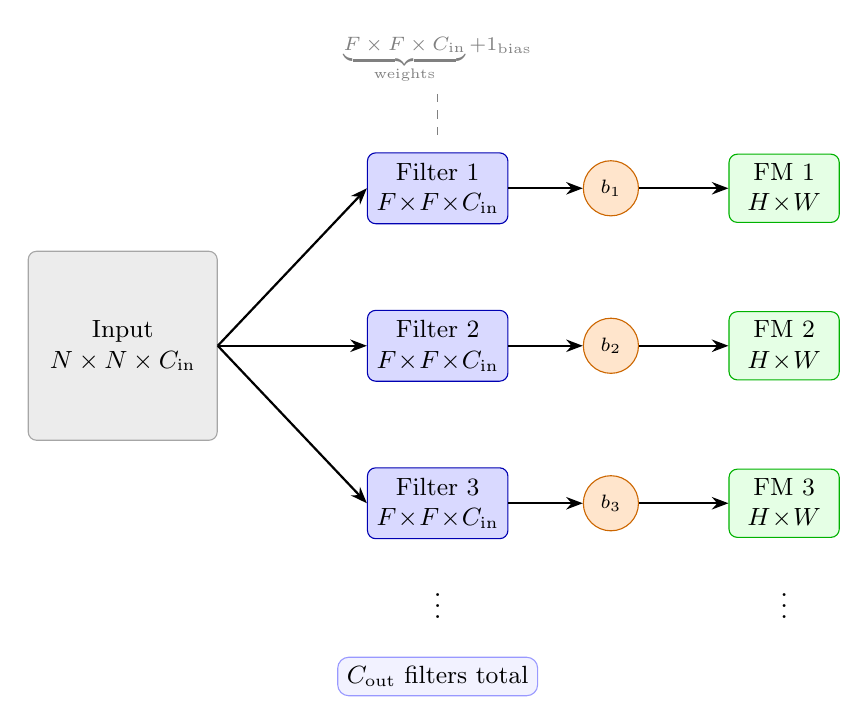
\begin{tikzpicture}[
  filter/.style={draw=blue!70!black, fill=blue!15, rounded corners=3pt,
                 minimum width=1.6cm, minimum height=0.9cm, font=\small},
  input/.style={draw=gray!70, fill=gray!15, rounded corners=3pt,
                minimum width=2.4cm, minimum height=2.4cm, font=\small},
  bias/.style={draw=orange!80!black, fill=orange!20, circle,
               minimum size=0.7cm, font=\scriptsize},
  arrow/.style={-{Stealth[length=6pt]}, thick},
  every node/.style={align=center}
]

%% Input volume
\node[input] (inp) at (0,0) {Input\\$N\times N\times\Cin$};

%% Three representative filters
\foreach \i/\y in {1/2.0, 2/0, 3/-2.0}{
  \node[filter] (f\i) at (4.0,\y) {Filter $\i$\\$F\!\times\!F\!\times\!\Cin$};
  \node[bias]   (b\i) at (6.2,\y) {$b_\i$};
  \draw[arrow] (inp.east) -- (f\i.west);
  \draw[arrow] (f\i.east) -- (b\i.west);
}

%% Output feature maps
\foreach \i/\y in {1/2.0, 2/0, 3/-2.0}{
  \node[draw=green!70!black, fill=green!10, rounded corners=3pt,
        minimum width=1.4cm, minimum height=0.8cm, font=\small]
        (o\i) at (8.4,\y) {FM $\i$\\$H\!\times\!W$};
  \draw[arrow] (b\i.east) -- (o\i.west);
}

%% Ellipsis
\node at (4.0,-3.2) {$\vdots$};
\node at (8.4,-3.2) {$\vdots$};

%% Label: Cout filters total
\node[draw=blue!40, fill=blue!5, rounded corners=4pt,
      font=\small, minimum width=2.0cm]
     at (4.0,-4.2) {$\Cout$ filters total};

%% Annotation arrows
\draw[dashed, gray] (4.0, 3.2) -- (4.0, 2.6)
  node[above, font=\scriptsize, at start]
  {$\underbrace{F\times F\times\Cin}_{\text{weights}} + 1_{\text{bias}}$};

\end{tikzpicture}
\caption{Weight-sharing in a convolutional layer. Each of the $\Cout$ filters
  has $F \times F \times \Cin$ weight parameters and one bias, giving
  $(F^2 \Cin + 1)\Cout$ total parameters. All output locations share the same
  filter weights.}
\label{fig:param_count}
\end{figure}

\subsection{Algorithm: Computing Parameters Programmatically}

\Cref{alg:param_count} provides a systematic procedure for counting
parameters across a full CNN.

\begin{algorithm}[ht]
\DontPrintSemicolon
\caption{Count Trainable Parameters in a CNN}
\label{alg:param_count}
\KwIn{CNN model with layers $\ell = 1, \ldots, L$}
\KwOut{Total parameter count $P_{\mathrm{total}}$}

$P_{\mathrm{total}} \leftarrow 0$\;
\For{each layer $\ell$ in model}{
  \uIf{$\ell$ is \texttt{Conv2d}($\Cin$, $\Cout$, $F$, \texttt{bias}$=b$)}{
    $P_\ell \leftarrow F \times F \times \Cin \times \Cout$\;
    \If{$b = \mathrm{True}$}{
      $P_\ell \leftarrow P_\ell + \Cout$
        \tcp*{one bias per output filter}
    }
  }
  \uElseIf{$\ell$ is \texttt{Linear}($d_{\mathrm{in}}$, $d_{\mathrm{out}}$, \texttt{bias}$=b$)}{
    $P_\ell \leftarrow d_{\mathrm{in}} \times d_{\mathrm{out}}$\;
    \If{$b = \mathrm{True}$}{
      $P_\ell \leftarrow P_\ell + d_{\mathrm{out}}$
    }
  }
  \uElseIf{$\ell$ is \texttt{BatchNorm2d}($C$)}{
    $P_\ell \leftarrow 2C$
      \tcp*{scale $\gamma$ and shift $\beta$, one per channel}
  }
  \Else{
    $P_\ell \leftarrow 0$
      \tcp*{Activation, Pooling, Dropout have no parameters}
  }
  $P_{\mathrm{total}} \leftarrow P_{\mathrm{total}} + P_\ell$\;
}
\Return $P_{\mathrm{total}}$\;
\end{algorithm}

\subsection{Comparison: Conv2d vs Fully-Connected Layer}

A critical insight from the session is that weight sharing makes CNNs
dramatically more parameter-efficient than fully-connected (FC) layers for
the same representational task.

\begin{keyinsight}
For a 128-channel $7 \times 7$ feature map fed into 64 units:
\begin{align*}
  P_{\mathrm{conv}} &= (3 \times 3 \times 128 + 1) \times 64 = 73{,}792 \\
  P_{\mathrm{FC}}   &= (7 \times 7 \times 128 + 1) \times 64
                     = (6272 + 1) \times 64 = 401{,}472
\end{align*}
The convolutional layer uses roughly $\mathbf{5.4\times}$ fewer parameters
while scanning the entire $7 \times 7$ spatial grid.
\end{keyinsight}

\begin{table}[ht]
  \centering
  \caption{Parameter comparison: \texttt{Conv2d} vs \texttt{Linear} for
    equivalent channel transformation ($\Cin=128$, $\Cout=64$).}
  \label{tab:param_comparison}
  \begin{tabularx}{\linewidth}{@{}Xrrr@{}}
    \toprule
    Layer type & Weight params & Bias params & \textbf{Total} \\
    \midrule
    \texttt{Conv2d(128,64,3)} no bias
      & $3\!\times\!3\!\times\!128\!\times\!64 = 73{,}728$  & 0 & 73,728 \\
    \texttt{Conv2d(128,64,3)} with bias
      & $73{,}728$  & 64 & \textbf{73,792} \\
    \texttt{Conv2d(128,64,5)} with bias
      & $5\!\times\!5\!\times\!128\!\times\!64 = 204{,}800$ & 64 & 204,864 \\
    \texttt{Linear(6272,64)} with bias
      & $7\!\times\!7\!\times\!128\!\times\!64 = 401{,}408$ & 64 & 401,472 \\
    \texttt{Linear(6272,64)} no bias
      & $401{,}408$ & 0 & 401,408 \\
    \bottomrule
  \end{tabularx}
\end{table}

% ════════════════════════════════════════════════════════════════════════════
\section{Convolution Output Size Formula}
\label{sec:output_size}
% ════════════════════════════════════════════════════════════════════════════

\subsection{General Formula}

The spatial dimension of the output feature map for a single axis is:

\begin{equation}
  \label{eq:output_size}
  H_{\mathrm{out}} = \floor{\frac{N - F + 2P}{S}} + 1
\end{equation}

The formula is symmetric in height and width when the input is square and
the kernel is square (which is the overwhelmingly common case). For
non-square inputs, height and width are treated independently.

\begin{definition}[Same Padding]
\label{def:same_padding}
``Same'' padding refers to the choice of $P$ such that
$H_{\mathrm{out}} = N$ when $S = 1$. Solving
\cref{eq:output_size} with $H_{\mathrm{out}} = N$ and $S = 1$:
\[
  N = \frac{N - F + 2P}{1} + 1
  \;\Longrightarrow\;
  P = \frac{F - 1}{2}
\]
This requires $F$ to be odd (the standard practice: $F \in \{1, 3, 5, 7\}$).
\end{definition}

\subsection{Common Configurations}

\Cref{tab:output_size_configs} tabulates the most common padding and stride
configurations encountered in practice.

\begin{table}[ht]
  \centering
  \caption{Output size formulae for common \texttt{Conv2d} configurations.
    Input: $N \times N$, filter $F \times F$.}
  \label{tab:output_size_configs}
  \begin{tabular}{@{}llll@{}}
    \toprule
    Configuration & Padding $P$ & Stride $S$ & Output size \\
    \midrule
    \multirow{2}{*}{No padding (``valid'')}
      & \multirow{2}{*}{0} & 1 & $N - F + 1$ \\
      &                    & 2 & $\floor{(N-F)/2}+1$ \\[4pt]
    \multirow{2}{*}{Same padding (preserve size)}
      & \multirow{2}{*}{$(F-1)/2$} & 1 & $N$ \\
      &                            & 2 & $\floor{N/2}$ \\[4pt]
    Strided (halve spatial dims) & 0 & 2 & $\floor{(N-F)/2}+1 \approx N/2$ \\
    \bottomrule
  \end{tabular}
\end{table}

\subsection{Worked Examples}

\begin{example}[title=Output sizes for a $7 \times 7$ input]
Let $N = 7$.

\medskip
\begin{tabular}{@{}llcl@{}}
  \toprule
  Layer & $(F, P, S)$ & Formula & Output \\
  \midrule
  \texttt{Conv2d(..., 3, padding=0)} & $(3,0,1)$
    & $\floor{(7-3+0)/1}+1$ & $5 \times 5$ \\
  \texttt{Conv2d(..., 3, padding=1)} & $(3,1,1)$
    & $\floor{(7-3+2)/1}+1$ & $7 \times 7$ \\
  \texttt{Conv2d(..., 3, stride=2)}  & $(3,0,2)$
    & $\floor{(7-3+0)/2}+1$ & $3 \times 3$ \\
  \texttt{Conv2d(..., 5, padding=2)} & $(5,2,1)$
    & $\floor{(7-5+4)/1}+1$ & $7 \times 7$ \\
  \bottomrule
\end{tabular}
\end{example}

\begin{example}[title=VGG-style block: $224 \to 112$]
A common pattern in VGG and similar networks uses a $3 \times 3$ conv with
same padding followed by a $2 \times 2$ max-pool with stride 2:

\begin{align*}
  \text{After conv (same)}: &\quad 224 \times 224 \\
  \text{After pool (stride 2)}: &\quad \floor{224/2} \times \floor{224/2}
    = 112 \times 112
\end{align*}

Each pooling stage halves the spatial dimensions while the number of
channels is doubled by the subsequent conv block.
\end{example}

\subsection{TikZ Diagram: Convolution Output Size}

\begin{figure}[ht]
\centering
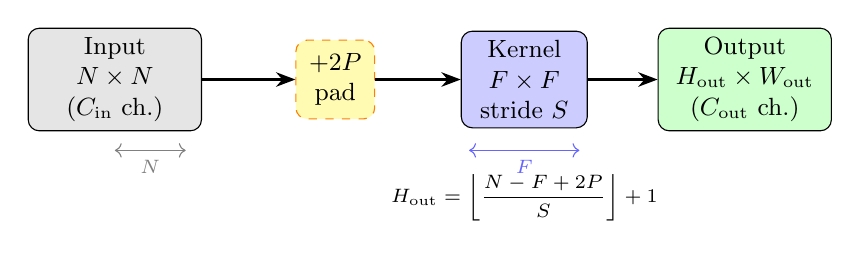
\begin{tikzpicture}[
  box/.style={draw, fill=#1, rounded corners=4pt, minimum height=1.0cm,
              font=\small, align=center},
  label/.style={font=\scriptsize, align=center},
  arrow/.style={-{Stealth[length=7pt]}, thick}
]

%% Input grid (5x5 shown as block)
\node[box=gray!20, minimum width=2.2cm] (inp) at (0,0)
  {Input\\$N \times N$\\$(\Cin$ ch.)};

%% Padding annotation
\node[box=yellow!30, minimum width=1.0cm, minimum height=1.0cm,
      dashed, draw=orange] (pad) at (2.8,0)
  {$+2P$\\pad};

%% Kernel
\node[box=blue!20, minimum width=1.6cm] (kern) at (5.2,0)
  {Kernel\\$F \times F$\\stride $S$};

%% Output
\node[box=green!20, minimum width=2.2cm] (out) at (8.0,0)
  {Output\\$H_{\mathrm{out}} \times W_{\mathrm{out}}$\\$(\Cout$ ch.)};

\draw[arrow] (inp.east) -- (pad.west);
\draw[arrow] (pad.east) -- (kern.west);
\draw[arrow] (kern.east) -- (out.west);

%% Formula below
\node[label] at (5.2,-1.5)
  {$H_{\mathrm{out}} = \left\lfloor\dfrac{N - F + 2P}{S}\right\rfloor + 1$};

%% Annotations
\draw[<->, gray, thin] (0,-0.9) -- node[below, font=\scriptsize]{$N$} (0.9,-0.9);
\draw[<->, blue!60, thin] (4.5,-0.9)
  -- node[below, font=\scriptsize]{$F$} (5.9,-0.9);

\end{tikzpicture}
\caption{Schematic of the convolution output size computation.
  Padding $P$ enlarges the effective input, the kernel of size $F$ slides
  across it with stride $S$, and the floor operation accounts for the
  integer number of complete strides.}
\label{fig:output_size}
\end{figure}

\begin{warningbox}
A common error is to forget the $+1$ term in \cref{eq:output_size}. This
term counts the initial filter placement at position 0 before any stride
steps are taken. Without it, the formula underestimates the output size by 1
in each spatial dimension. For a $5 \times 5$ input with a $3 \times 3$
filter and no padding: $\floor{(5-3)/1}+1 = 3$, not 2.
\end{warningbox}

% ════════════════════════════════════════════════════════════════════════════
\section{L2 Regularisation and Weight Decay}
\label{sec:l2reg}
% ════════════════════════════════════════════════════════════════════════════

\subsection{Motivation: Overfitting and Generalisation}

When a neural network has many more parameters than training samples, or
when training runs for many epochs, it can memorise the training data rather
than learning transferable features. This phenomenon---\emph{overfitting}---
manifests as low training loss but high validation/test loss.

Regularisation adds a penalty term to the loss that discourages excessively
large weights, biasing the optimiser toward solutions that generalise better.

\subsection{Mathematical Formulation}

\begin{definition}[L2 Regularised Loss]
\label{def:l2_loss}
The L2 regularised total loss is:
\begin{equation}
  \label{eq:l2_loss}
  \Ltotal = \Ldata + \lambda \sum_{i} w_i^2
\end{equation}
where $\Ldata$ is the task loss (cross-entropy, MSE, etc.),
$w_i$ are the learnable weight parameters (biases are typically excluded),
and $\lambda > 0$ is the regularisation strength.
\end{definition}

The penalty $\lambda \sum_i w_i^2$ penalises large-magnitude weights
quadratically, so the optimiser is incentivised to keep all weights small
unless forced large by the data loss.

\subsection{Gradient Update with L2 Penalty}

Taking the gradient of \cref{eq:l2_loss} with respect to a single weight
$w$:

\begin{align}
  \frac{\partial \Ltotal}{\partial w}
    &= \frac{\partial \Ldata}{\partial w} + 2\lambda w
  \label{eq:l2_grad}
\end{align}

The standard gradient descent update then becomes:

\begin{align}
  w &\leftarrow w - \eta \frac{\partial \Ltotal}{\partial w} \notag \\
    &= w - \eta \left(\frac{\partial \Ldata}{\partial w} + 2\lambda w\right)
       \notag \\
    &= w\bigl(1 - 2\eta\lambda\bigr)
       - \eta \frac{\partial \Ldata}{\partial w}
  \label{eq:weight_decay_update}
\end{align}

\begin{keyinsight}
\Cref{eq:weight_decay_update} reveals why L2 regularisation is also called
\textbf{weight decay}: the factor $(1 - 2\eta\lambda)$ \emph{decays} every
weight toward zero at each step, regardless of the gradient. The data
gradient then ``pushes back'' to maintain useful representations. The
balance between decay and push-back determines the effective magnitude of
learned weights.
\end{keyinsight}

\subsection{The Factor-of-Two Convention}

During the session, students raised the question of whether the gradient
update involves $2\lambda$ or $\lambda$. This depends on which convention
is used for the penalty:

\begin{align}
  \text{Convention A (standard):}\quad
    &\mathcal{L}_{\mathrm{reg}} = \lambda \sum_i w_i^2
    &&\Rightarrow\; \nabla_w \mathcal{L}_{\mathrm{reg}} = 2\lambda w
    \label{eq:conv_a} \\[4pt]
  \text{Convention B (divided by 2):}\quad
    &\mathcal{L}_{\mathrm{reg}} = \frac{\lambda}{2} \sum_i w_i^2
    &&\Rightarrow\; \nabla_w \mathcal{L}_{\mathrm{reg}} = \lambda w
    \label{eq:conv_b}
\end{align}

\noindent
The instructors confirmed that exam questions follow \textbf{Convention A}
unless the question explicitly provides a formula with $\tfrac{1}{2}$.
Students should read the question statement carefully and use whichever form
is given.

\begin{remark}
\label{rem:pytorch_convention}
PyTorch's \texttt{weight\_decay} parameter in SGD and Adam implements
\emph{weight decay} directly (multiplying weights by $(1-\eta\lambda_{\mathrm{wd}})$
per step), which corresponds to Convention B at the gradient level. For most
practical purposes the distinction does not matter because $\lambda$ is
tuned empirically. However, for numeric exam questions, one must use the
exact formula provided.
\end{remark}

\subsection{PyTorch Implementation}

L2 regularisation is activated by passing a non-zero \texttt{weight\_decay}
argument to any PyTorch optimiser:

\begin{verbatim}
import torch.optim as optim

# Adam with L2 regularisation (weight_decay acts as lambda)
optimizer = optim.Adam(model.parameters(),
                       lr=1e-3,
                       weight_decay=1e-4)   # lambda = 0.0001

# SGD with weight decay and momentum
optimizer = optim.SGD(model.parameters(),
                      lr=1e-1,
                      weight_decay=1e-4,
                      momentum=0.9)
\end{verbatim}

\noindent
\textbf{Default:} \texttt{weight\_decay=0}, meaning no regularisation is
applied unless explicitly set.

\subsection{Effect on the Loss Surface}

Adding the L2 term reshapes the optimisation landscape. The effective loss
becomes a sum of the data loss and a bowl-shaped quadratic. This has three
practical consequences:

\begin{enumerate}[label=\textbf{(\roman*)}]
  \item \textbf{Unique minimum}: Even if $\Ldata$ has flat directions (e.g.,
        under-determined systems), the L2 term creates a unique minimum at
        $\mathbf{w} = \mathbf{0}$ in the absence of data.
  \item \textbf{Smaller weights}: The optimal weights are pulled toward zero
        relative to the unregularised solution.
  \item \textbf{Smoother decision boundaries}: Smaller weights in
        classification networks imply flatter activation surfaces, reducing
        the risk of sharp spurious boundaries that do not generalise.
\end{enumerate}

\begin{table}[ht]
  \centering
  \caption{Effect of \texttt{weight\_decay} (L2 regularisation strength) on
    model behaviour. Typical experimental observations.}
  \label{tab:l2_effect}
  \begin{tabularx}{\linewidth}{@{}lXX@{}}
    \toprule
    \texttt{weight\_decay} & Effect on training & Effect on generalisation \\
    \midrule
    $0$ (default)
      & Weights grow freely; fast convergence on training set
      & Risk of overfitting; poor test performance if data is scarce \\
    $10^{-4}$ (light)
      & Slight weight shrinkage; negligible training loss impact
      & Small generalisation improvement; common default choice \\
    $10^{-3}$ (moderate)
      & Noticeable weight shrinkage; may slow convergence
      & Better generalisation; can under-fit if combined with small model \\
    $10^{-2}$ (strong)
      & Heavy weight shrinkage; training loss visibly higher
      & Strong bias toward zero weights; often too aggressive \\
    \bottomrule
  \end{tabularx}
\end{table}

% ════════════════════════════════════════════════════════════════════════════
\section{Comparative Analysis and Design Decisions}
\label{sec:comparison}
% ════════════════════════════════════════════════════════════════════════════

\subsection{Parameter Efficiency: Conv vs FC vs Depthwise Conv}

To place Session 15's parameter-counting exercise in a broader context,
\cref{tab:arch_comparison} compares several layer types for the
same $\Cin = 128$, $\Cout = 64$ transformation.

\begin{table}[ht]
  \centering
  \caption{Parameter counts for different layer types with
    $\Cin=128$, $\Cout=64$, $F=3$.}
  \label{tab:arch_comparison}
  \begin{tabularx}{\linewidth}{@{}Xrrl@{}}
    \toprule
    Layer type & Weight params & Bias & Total \\
    \midrule
    \texttt{Conv2d(128,64,3)} (standard)
      & 73,728 & 64 & 73,792 \\
    \texttt{Conv2d(128,64,1)} ($1\times1$ conv)
      & 8,192  & 64 & 8,256 \\
    Depthwise \texttt{Conv2d(128,128,3)} + pointwise
      & $9\times128 + 128\times64 = 1152+8192$
      & $128+64$ & 9,536 \\
    \texttt{Linear(128,64)} (no spatial)
      & 8,192 & 64 & 8,256 \\
    \texttt{Linear(7$\times$7$\times$128, 64)} (flattened)
      & 401,408 & 64 & 401,472 \\
    \bottomrule
  \end{tabularx}
\end{table}

\noindent
The depthwise-separable factorisation used in MobileNet achieves roughly the
same representation with $\sim$8$\times$ fewer parameters than standard
\texttt{Conv2d}.

\subsection{Regularisation Strategies: L2 vs Dropout vs Batch Norm}

L2 regularisation is one of several complementary strategies available in
deep learning. \Cref{tab:reg_comparison} provides a side-by-side comparison.

\begin{table}[ht]
  \centering
  \caption{Comparison of regularisation strategies.}
  \label{tab:reg_comparison}
  \begin{tabularx}{\linewidth}{@{}lXXX@{}}
    \toprule
    Technique & Mechanism & Hyperparameter & Typical use \\
    \midrule
    L2 (weight decay)
      & Penalises large weights; shrinks weights toward zero
      & \texttt{weight\_decay} $\lambda$
      & Almost always used; \texttt{1e-4} default \\
    L1 regularisation
      & Penalises absolute weight magnitude; encourages sparsity
      & Regularisation coefficient
      & Sparse models, feature selection \\
    Dropout
      & Randomly zeros activations during training
      & Drop probability $p$
      & FC layers; \texttt{p=0.5} classic \\
    Batch Normalisation
      & Normalises layer inputs; implicit regularisation
      & Momentum, $\epsilon$
      & Between conv and activation \\
    Data Augmentation
      & Expands effective training set via transforms
      & Augmentation policy
      & Image tasks; near-zero cost \\
    Early Stopping
      & Halts training when validation loss increases
      & Patience epochs
      & Universal safety net \\
    \bottomrule
  \end{tabularx}
\end{table}

\subsection{Padding Regime Tradeoffs}

\begin{keyinsight}
The choice of padding regime affects both the output spatial dimension and
the receptive field coverage at the feature map borders:
\begin{itemize}[noitemsep]
  \item \textbf{Valid padding ($P=0$)}: Spatial dimensions shrink with depth;
        border pixels appear in fewer filter applications. Used in LeNet-5
        and early CNNs.
  \item \textbf{Same padding ($P=(F{-}1)/2$)}: Spatial dimensions preserved;
        all positions receive equal filter coverage. Used in VGG, ResNet,
        and modern architectures.
  \item \textbf{Strided convolution ($S=2$, $P=0$)}: Spatial downsampling
        without pooling; the stride itself performs subsampling. Preferred in
        modern efficient architectures (e.g., ResNet stem, DCGAN generator).
\end{itemize}
\end{keyinsight}

% ════════════════════════════════════════════════════════════════════════════
\section{Unified TikZ Architecture Diagram}
\label{sec:architecture}
% ════════════════════════════════════════════════════════════════════════════

\Cref{fig:cnn_pipeline} shows the full computation pipeline for a single
convolutional block, annotating where the output size formula
(\cref{eq:output_size}) and parameter count formula (\cref{eq:param_formula})
apply.

\begin{figure}[ht]
\centering
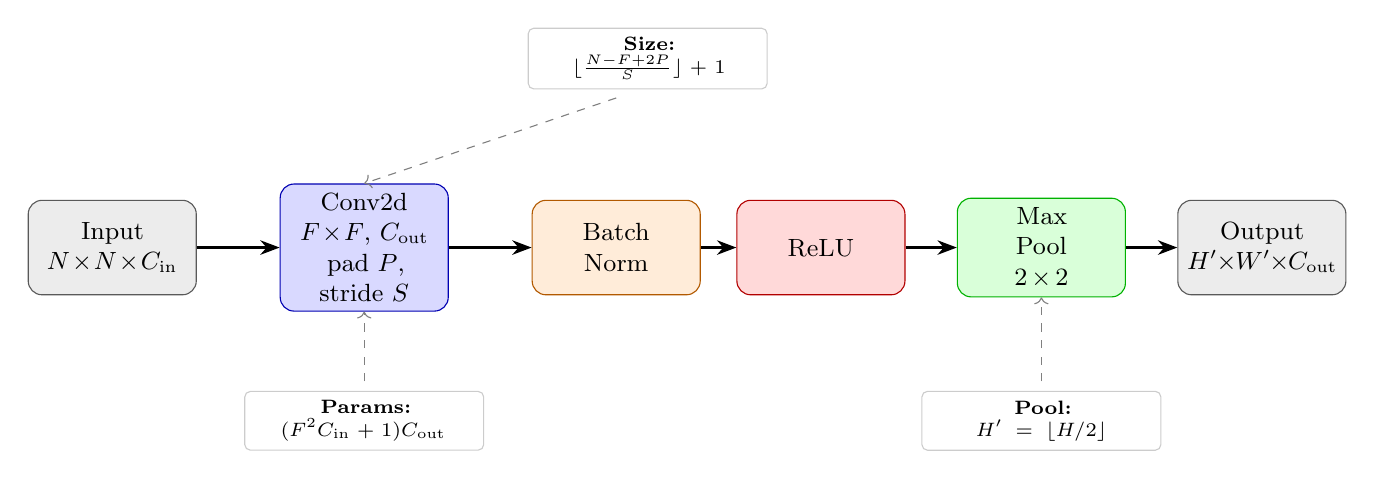
\begin{tikzpicture}[
  blk/.style={draw=#1!70!black, fill=#1!15, rounded corners=5pt,
              minimum width=2.0cm, minimum height=1.2cm,
              font=\small, align=center, text width=1.9cm},
  ann/.style={font=\scriptsize, draw=gray!40, fill=white,
              rounded corners=2pt, align=center, text width=2.8cm},
  arrow/.style={-{Stealth[length=7pt]}, thick, #1},
  every node/.style={align=center}
]

%% Nodes left to right
\node[blk=gray]   (inp)  at (0,   0) {Input\\$N\!\times\!N\!\times\!\Cin$};
\node[blk=blue]   (conv) at (3.2, 0) {Conv2d\\$F\!\times\!F$, $\Cout$\\pad $P$, stride $S$};
\node[blk=orange] (bn)   at (6.4, 0) {Batch\\Norm};
\node[blk=red]    (act)  at (9.0, 0) {ReLU};
\node[blk=green]  (pool) at (11.8,0) {Max\\Pool\\$2\!\times\!2$};
\node[blk=gray]   (out)  at (14.6,0) {Output\\$H'\!\times\!W'\!\times\!\Cout$};

%% Arrows
\draw[arrow={}] (inp.east)  -- (conv.west);
\draw[arrow={}] (conv.east) -- (bn.west);
\draw[arrow={}] (bn.east)   -- (act.west);
\draw[arrow={}] (act.east)  -- (pool.west);
\draw[arrow={}] (pool.east) -- (out.west);

%% Annotation: parameter count
\node[ann] at (3.2, -2.2)
  {\textbf{Params:}\\$(F^2\Cin+1)\Cout$};
\draw[->, dashed, gray] (3.2,-1.7) -- (conv.south);

%% Annotation: output size
\node[ann] at (6.8, 2.4)
  {\textbf{Size:}\\$\lfloor\frac{N-F+2P}{S}\rfloor+1$};
\draw[->, dashed, gray] (6.4,1.9) -- (conv.north);

%% Annotation: pool halves
\node[ann] at (11.8,-2.2)
  {\textbf{Pool:}\\$H' = \lfloor H/2\rfloor$};
\draw[->, dashed, gray] (11.8,-1.7) -- (pool.south);

\end{tikzpicture}
\caption{Typical CNN convolutional block pipeline. The parameter count
  formula applies at the \texttt{Conv2d} step; the output size formula
  applies at both \texttt{Conv2d} and \texttt{MaxPool2d}. BatchNorm and
  ReLU do not change spatial dimensions and have no (or negligible) learnable
  parameters.}
\label{fig:cnn_pipeline}
\end{figure}

% ════════════════════════════════════════════════════════════════════════════
\section{Session Q\&A: Detailed Walkthroughs}
\label{sec:qa}
% ════════════════════════════════════════════════════════════════════════════

This section provides extended solutions to the questions raised during
Session 15.

\subsection{Q1: Counting Parameters with Bias}

\textbf{Question (paraphrased from session):} \\
\textit{A convolution layer has 64 filters, kernel size $3 \times 3$, and
128 input channels. Should we include bias? How many parameters total?}

\textbf{Answer:} \\
Yes, bias is included by default in PyTorch (\texttt{bias=True}). Using
\cref{eq:param_formula}:

\begin{align*}
  P &= (F^2 \cdot \Cin + 1) \cdot \Cout \\
    &= (9 \cdot 128 + 1) \cdot 64 \\
    &= 1153 \cdot 64 \\
    &= \mathbf{73{,}792}
\end{align*}

\textbf{Choice of correct answer:} If the multiple-choice options include
both $73{,}728$ (no bias) and $73{,}792$ (with bias), and the question does
not specify \texttt{bias=False}, select $73{,}792$.

\subsection{Q2: L2 Penalty Contribution --- Theory vs PyTorch}

\textbf{Question (paraphrased from session):} \\
\textit{Given weight decay $\lambda = 10^{-4}$ and weights
$\mathbf{w} = [w_1, w_2, \ldots]$, what is the L2 penalty contribution to
the loss? There seem to be two formulas (theoretical and PyTorch). Which do
we use?}

\textbf{Answer:} \\
For exam purposes, use the \textbf{theoretical formula}:
\begin{equation}
  \mathcal{L}_{\mathrm{L2}} = \lambda \sum_i w_i^2
  \label{eq:l2_penalty_qa}
\end{equation}

If the exam question provides a formula that includes $\tfrac{1}{2}$:
\[
  \mathcal{L}_{\mathrm{L2}} = \frac{\lambda}{2} \sum_i w_i^2
\]
then use \emph{that} formula instead and do \emph{not} include the factor
of 2 in the gradient. The key signal is: \textbf{use whichever formula is
given in the question}.

\textbf{Numerical example:} With $\lambda = 10^{-4}$ and weights
$\mathbf{w} = [0.5, -0.3, 0.8]$:
\begin{align*}
  \sum_i w_i^2 &= 0.25 + 0.09 + 0.64 = 0.98 \\
  \mathcal{L}_{\mathrm{L2}} &= 10^{-4} \times 0.98 = 9.8 \times 10^{-5}
\end{align*}

\subsection{Q3: Output Size for Standard Layers}

\textbf{Question:} \\
\textit{What is the output size after \texttt{Conv2d(128, 64, kernel\_size=3,
stride=1, padding=0)} applied to a $7 \times 7$ feature map?}

\textbf{Answer:} Using \cref{eq:output_size} with $N=7$, $F=3$, $P=0$,
$S=1$:
\[
  H_{\mathrm{out}} = \floor{\frac{7 - 3 + 0}{1}} + 1 = 4 + 1 = \mathbf{5}
\]
Output: $5 \times 5 \times 64$.

% ════════════════════════════════════════════════════════════════════════════
\section{Transition to Recurrent Neural Networks}
\label{sec:rnn_preview}
% ════════════════════════════════════════════════════════════════════════════

Session 15 marks the end of the CNN module and the beginning of the
transition to \textbf{Recurrent Neural Networks} (RNNs), covered by the
\texttt{08\_PyTorchDL\_RNN} deck. This section briefly previews the
conceptual shift.

\subsection{Limitations of CNNs for Sequential Data}

CNNs operate on fixed-size inputs with no inherent notion of \emph{temporal
order}. When the input is a sequence (text, speech, time series), CNNs can
capture local patterns within a window via 1D convolutions, but they
\begin{itemize}[noitemsep]
  \item Cannot maintain \emph{state} across time steps,
  \item Require a fixed receptive field (context window), and
  \item Do not model variable-length dependencies.
\end{itemize}

\subsection{The RNN Paradigm}

RNNs address these limitations by introducing a \emph{hidden state}
$\mathbf{h}_t$ that is updated at each time step $t$:

\begin{equation}
  \mathbf{h}_t = \tanh\!\left(W_{hh}\,\mathbf{h}_{t-1}
                             + W_{xh}\,\mathbf{x}_t + \mathbf{b}\right)
  \label{eq:rnn_cell}
\end{equation}

where $\mathbf{x}_t$ is the input at step $t$, and
$W_{hh}$, $W_{xh}$, $\mathbf{b}$ are shared parameters across all time
steps (analogous to weight sharing in CNNs).

\begin{keyinsight}
The same weight matrices $(W_{hh}, W_{xh})$ are applied at every time step,
just as the same filter weights are applied at every spatial location in a
CNN. This is the RNN analogue of \textbf{weight sharing across time}.
\end{keyinsight}

\begin{table}[ht]
  \centering
  \caption{CNN vs RNN conceptual comparison.}
  \label{tab:cnn_vs_rnn}
  \begin{tabularx}{\linewidth}{@{}lXX@{}}
    \toprule
    Concept & CNN (spatial) & RNN (temporal) \\
    \midrule
    Input structure   & Grid ($H \times W \times C$)
                      & Sequence ($T \times d$) \\
    Shared parameters & Filter weights across spatial locations
                      & Weight matrices across time steps \\
    State             & Feature maps (static)
                      & Hidden state $\mathbf{h}_t$ (evolves) \\
    Inductive bias    & Local spatial patterns
                      & Temporal dependencies \\
    Depth             & Number of stacked conv layers
                      & Sequence length (unrolled depth) \\
    Gradient issue    & Vanishing gradients (deep nets)
                      & Vanishing/exploding gradients (long sequences) \\
    \bottomrule
  \end{tabularx}
\end{table}

\noindent
The RNN module will cover vanilla RNNs, Long Short-Term Memory (LSTM) cells,
and Gated Recurrent Units (GRUs), building on the same parameter-counting
and regularisation foundations established in the CNN module.

% ════════════════════════════════════════════════════════════════════════════
\section{Summary and Conclusions}
\label{sec:conclusion}
% ════════════════════════════════════════════════════════════════════════════

Session 15 served as a focused consolidation session before transitioning
to the RNN module. The three core topics revisited and clarified were:

\begin{enumerate}[label=\textbf{(\arabic*)}, leftmargin=2em]

  \item \textbf{Convolutional layer parameter counting}
    (\cref{sec:param_count}): The formula
    $(F^2 \cdot \Cin + 1) \cdot \Cout$ gives the exact number of trainable
    parameters in a \texttt{Conv2d} layer, \emph{independent of the input
    spatial size}. For the exam example of 64 filters, $3\times3$ kernels,
    128 input channels, the answer is \textbf{73,792} with bias (73,728
    without). This is $\sim$$5.4\times$ fewer than the equivalent fully-connected
    layer ($\sim$401,472), illustrating the efficiency of weight sharing.

  \item \textbf{Convolution output size formula}
    (\cref{sec:output_size}): The general formula is
    $\floor{(N - F + 2P)/S} + 1$. The three key configurations are
    \emph{valid} ($P=0$), \emph{same} ($P=(F{-}1)/2$, preserves size for
    odd $F$), and \emph{strided} ($S=2$, halves spatial dimensions). The
    $+1$ term is frequently omitted in error and must always be included.

  \item \textbf{L2 regularisation and weight decay}
    (\cref{sec:l2reg}): The regularised loss
    $\Ldata + \lambda\sum_i w_i^2$ penalises large weights quadratically.
    The resulting gradient update $(1 - 2\eta\lambda)w -
    \eta\nabla_w\Ldata$ is called weight decay because it shrinks weights
    at every step. In PyTorch, this is controlled by the
    \texttt{weight\_decay} argument to any optimiser. For exam calculations,
    use the formula provided in the question---with or without the factor of
    $\tfrac{1}{2}$ depending on what is stated.

\end{enumerate}

\medskip

\noindent
\textbf{Preview of Session 16 (RNNs):}
The next session introduces Recurrent Neural Networks using the
\texttt{08\_PyTorchDL\_RNN} slide deck. The same principles of weight
sharing, parameter counting, and regularisation carry over, now applied
to sequences rather than spatial feature maps.

\begin{keyinsight}
Three formulae to commit to memory from Session 15:
\begin{align*}
  \text{Conv params:}\quad
    & P = (F^2 \cdot \Cin + 1) \cdot \Cout \\
  \text{Output size:}\quad
    & H_{\mathrm{out}} = \floor{\frac{N - F + 2P}{S}} + 1 \\
  \text{L2 loss:}\quad
    & \Ltotal = \Ldata + \lambda\sum_i w_i^2
\end{align*}
\end{keyinsight}

% ════════════════════════════════════════════════════════════════════════════
%  APPENDIX
% ════════════════════════════════════════════════════════════════════════════
\appendix

\section{Quick-Reference Formula Sheet}
\label{app:formulas}

\subsection*{Convolutional Layer --- Parameter Count}
\[
  P_{\mathrm{conv}} = (F \times F \times \Cin + b) \times \Cout,
  \quad b = \begin{cases}1 & \text{bias=True (default)}\\0 & \text{bias=False}\end{cases}
\]

\subsection*{Convolution Output Size}
\[
  H_{\mathrm{out}} = \floor{\frac{N - F + 2P}{S}} + 1
\]

\textbf{Special cases:}
\begin{itemize}[noitemsep]
  \item Same padding: $P = (F-1)/2$, $S=1$ $\Rightarrow$ $H_{\mathrm{out}} = N$
  \item Valid padding: $P=0$, $S=1$ $\Rightarrow$ $H_{\mathrm{out}} = N - F + 1$
  \item Stride-2 downsampling: $P=0$, $S=2$ $\Rightarrow$
        $H_{\mathrm{out}} = \floor{(N-F)/2} + 1$
\end{itemize}

\subsection*{L2 Regularised Loss and Gradient}
\begin{align*}
  \Ltotal &= \Ldata + \lambda \sum_i w_i^2 \\
  \frac{\partial \Ltotal}{\partial w} &= \frac{\partial \Ldata}{\partial w} + 2\lambda w \\
  w &\leftarrow w\,(1 - 2\eta\lambda)
    - \eta\,\frac{\partial \Ldata}{\partial w}
\end{align*}

\subsection*{Typical Hyperparameter Ranges}
\begin{center}
\begin{tabular}{@{}lll@{}}
  \toprule
  Hyperparameter & Symbol & Typical range \\
  \midrule
  Learning rate (SGD)      & $\eta$ & $0.1$, $0.01$, $0.001$ \\
  Learning rate (Adam)     & $\eta$ & $10^{-3}$ \\
  Weight decay (L2)        & $\lambda$ & $10^{-4}$--$10^{-2}$ \\
  Momentum                 & $\mu$ & $0.9$ \\
  Dropout probability      & $p$ & $0.3$--$0.5$ \\
  \bottomrule
\end{tabular}
\end{center}

\section{Session Metadata}
\label{app:metadata}

\begin{center}
\begin{tabular}{@{}ll@{}}
  \toprule
  Field & Value \\
  \midrule
  Session       & 15 \\
  Format        & Interactive Q\&A / doubt-clearing \\
  Duration      & $\approx$ 1 hour 10 minutes \\
  Instructors   & Prof.\ S.~R.~M.\ Prasanna, Dr.\ Sunil Saumya \\
  Institution   & IIIT Dharwad \\
  Slide deck    & \texttt{08\_PyTorchDL\_RNN} \\
  Video URL     & \url{https://vimeo.com/1153110691} \\
  Preceding topic & CNNs with PyTorch (Sessions 10--14) \\
  Following topic & Recurrent Neural Networks (Session 16+) \\
  Topics covered  & Conv param counting, output size, L2 regularisation \\
  \bottomrule
\end{tabular}
\end{center}

\clearpage

\end{document}
